% Options for packages loaded elsewhere
\PassOptionsToPackage{unicode}{hyperref}
\PassOptionsToPackage{hyphens}{url}
\PassOptionsToPackage{dvipsnames,svgnames*,x11names*}{xcolor}
%
\documentclass[
  12pt,
]{book}
\usepackage{lmodern}
\usepackage{amsmath}
\usepackage{ifxetex,ifluatex}
\ifnum 0\ifxetex 1\fi\ifluatex 1\fi=0 % if pdftex
  \usepackage[T1]{fontenc}
  \usepackage[utf8]{inputenc}
  \usepackage{textcomp} % provide euro and other symbols
  \usepackage{amssymb}
\else % if luatex or xetex
  \usepackage{unicode-math}
  \defaultfontfeatures{Scale=MatchLowercase}
  \defaultfontfeatures[\rmfamily]{Ligatures=TeX,Scale=1}
  \setmonofont[]{Source Code Pro}
\fi
% Use upquote if available, for straight quotes in verbatim environments
\IfFileExists{upquote.sty}{\usepackage{upquote}}{}
\IfFileExists{microtype.sty}{% use microtype if available
  \usepackage[]{microtype}
  \UseMicrotypeSet[protrusion]{basicmath} % disable protrusion for tt fonts
}{}
\makeatletter
\@ifundefined{KOMAClassName}{% if non-KOMA class
  \IfFileExists{parskip.sty}{%
    \usepackage{parskip}
  }{% else
    \setlength{\parindent}{0pt}
    \setlength{\parskip}{6pt plus 2pt minus 1pt}}
}{% if KOMA class
  \KOMAoptions{parskip=half}}
\makeatother
\usepackage{xcolor}
\IfFileExists{xurl.sty}{\usepackage{xurl}}{} % add URL line breaks if available
\IfFileExists{bookmark.sty}{\usepackage{bookmark}}{\usepackage{hyperref}}
\hypersetup{
  pdftitle={Notas Curso Básico R},
  pdfauthor={Tobías Chavarría},
  colorlinks=true,
  linkcolor=Maroon,
  filecolor=Maroon,
  citecolor=Blue,
  urlcolor=Blue,
  pdfcreator={LaTeX via pandoc}}
\urlstyle{same} % disable monospaced font for URLs
\usepackage{color}
\usepackage{fancyvrb}
\newcommand{\VerbBar}{|}
\newcommand{\VERB}{\Verb[commandchars=\\\{\}]}
\DefineVerbatimEnvironment{Highlighting}{Verbatim}{commandchars=\\\{\}}
% Add ',fontsize=\small' for more characters per line
\usepackage{framed}
\definecolor{shadecolor}{RGB}{248,248,248}
\newenvironment{Shaded}{\begin{snugshade}}{\end{snugshade}}
\newcommand{\AlertTok}[1]{\textcolor[rgb]{0.94,0.16,0.16}{#1}}
\newcommand{\AnnotationTok}[1]{\textcolor[rgb]{0.56,0.35,0.01}{\textbf{\textit{#1}}}}
\newcommand{\AttributeTok}[1]{\textcolor[rgb]{0.77,0.63,0.00}{#1}}
\newcommand{\BaseNTok}[1]{\textcolor[rgb]{0.00,0.00,0.81}{#1}}
\newcommand{\BuiltInTok}[1]{#1}
\newcommand{\CharTok}[1]{\textcolor[rgb]{0.31,0.60,0.02}{#1}}
\newcommand{\CommentTok}[1]{\textcolor[rgb]{0.56,0.35,0.01}{\textit{#1}}}
\newcommand{\CommentVarTok}[1]{\textcolor[rgb]{0.56,0.35,0.01}{\textbf{\textit{#1}}}}
\newcommand{\ConstantTok}[1]{\textcolor[rgb]{0.00,0.00,0.00}{#1}}
\newcommand{\ControlFlowTok}[1]{\textcolor[rgb]{0.13,0.29,0.53}{\textbf{#1}}}
\newcommand{\DataTypeTok}[1]{\textcolor[rgb]{0.13,0.29,0.53}{#1}}
\newcommand{\DecValTok}[1]{\textcolor[rgb]{0.00,0.00,0.81}{#1}}
\newcommand{\DocumentationTok}[1]{\textcolor[rgb]{0.56,0.35,0.01}{\textbf{\textit{#1}}}}
\newcommand{\ErrorTok}[1]{\textcolor[rgb]{0.64,0.00,0.00}{\textbf{#1}}}
\newcommand{\ExtensionTok}[1]{#1}
\newcommand{\FloatTok}[1]{\textcolor[rgb]{0.00,0.00,0.81}{#1}}
\newcommand{\FunctionTok}[1]{\textcolor[rgb]{0.00,0.00,0.00}{#1}}
\newcommand{\ImportTok}[1]{#1}
\newcommand{\InformationTok}[1]{\textcolor[rgb]{0.56,0.35,0.01}{\textbf{\textit{#1}}}}
\newcommand{\KeywordTok}[1]{\textcolor[rgb]{0.13,0.29,0.53}{\textbf{#1}}}
\newcommand{\NormalTok}[1]{#1}
\newcommand{\OperatorTok}[1]{\textcolor[rgb]{0.81,0.36,0.00}{\textbf{#1}}}
\newcommand{\OtherTok}[1]{\textcolor[rgb]{0.56,0.35,0.01}{#1}}
\newcommand{\PreprocessorTok}[1]{\textcolor[rgb]{0.56,0.35,0.01}{\textit{#1}}}
\newcommand{\RegionMarkerTok}[1]{#1}
\newcommand{\SpecialCharTok}[1]{\textcolor[rgb]{0.00,0.00,0.00}{#1}}
\newcommand{\SpecialStringTok}[1]{\textcolor[rgb]{0.31,0.60,0.02}{#1}}
\newcommand{\StringTok}[1]{\textcolor[rgb]{0.31,0.60,0.02}{#1}}
\newcommand{\VariableTok}[1]{\textcolor[rgb]{0.00,0.00,0.00}{#1}}
\newcommand{\VerbatimStringTok}[1]{\textcolor[rgb]{0.31,0.60,0.02}{#1}}
\newcommand{\WarningTok}[1]{\textcolor[rgb]{0.56,0.35,0.01}{\textbf{\textit{#1}}}}
\usepackage{longtable,booktabs}
\usepackage{calc} % for calculating minipage widths
% Correct order of tables after \paragraph or \subparagraph
\usepackage{etoolbox}
\makeatletter
\patchcmd\longtable{\par}{\if@noskipsec\mbox{}\fi\par}{}{}
\makeatother
% Allow footnotes in longtable head/foot
\IfFileExists{footnotehyper.sty}{\usepackage{footnotehyper}}{\usepackage{footnote}}
\makesavenoteenv{longtable}
\usepackage{graphicx}
\makeatletter
\def\maxwidth{\ifdim\Gin@nat@width>\linewidth\linewidth\else\Gin@nat@width\fi}
\def\maxheight{\ifdim\Gin@nat@height>\textheight\textheight\else\Gin@nat@height\fi}
\makeatother
% Scale images if necessary, so that they will not overflow the page
% margins by default, and it is still possible to overwrite the defaults
% using explicit options in \includegraphics[width, height, ...]{}
\setkeys{Gin}{width=\maxwidth,height=\maxheight,keepaspectratio}
% Set default figure placement to htbp
\makeatletter
\def\fps@figure{htbp}
\makeatother
\setlength{\emergencystretch}{3em} % prevent overfull lines
\providecommand{\tightlist}{%
  \setlength{\itemsep}{0pt}\setlength{\parskip}{0pt}}
\setcounter{secnumdepth}{5}
%\usepackage{inputenc}
% \usepackage{newpxtext,newpxmath}
\setcounter{tocdepth}{3}
\setcounter{secnumdepth}{3}
\usepackage[spanish]{babel}
\usepackage{booktabs}
\usepackage{csquotes}
\usepackage{amsmath, amsthm, amssymb,amsbsy}
\usepackage{mathtools}
\usepackage{graphics, graphicx}
\usepackage{listings}

\lstset{
	breaklines=true
}


% \usepackage{setspace}
% \doublespacing
%\addbibresource{bibliografia.bib}


% \usepackage{tcolorbox}
% \tcbuselibrary{theorems}
% \tcbuselibrary{breakable}
% 
% \newtcbtheorem[number within=section]{nota}{Nota}%
% {breakable, colback=yellow!5, colframe=yellow!40!gray,
% 	fonttitle=\bfseries}{nota}
% 
% \newtcbtheorem[number within=section,use counter
% from=nota]{cuidado}{Cuidado}%
% {breakable, colback=red!5, colframe=red!50!gray,
% 	fonttitle=\bfseries}{cuidado}
% 
% \newtcbtheorem[number within=section,use counter
% from=nota]{tarea}{Tarea}%
% {breakable, colback=blue!5, colframe=blue!35!black,
% 	fonttitle=\bfseries}{tarea}
% 
% \newtcbtheorem[number within=section,use counter
% from=nota]{solucion}{Solución}%
% {breakable, colback=gray!5, colframe=gray!35!black,
% 	fonttitle=\bfseries}{sol}
% 
% \newtcbtheorem[number within=section,use counter
% from=nota]{pregunta}{Pregunta}%
% {breakable,  colback=green!5, colframe=green!35!black,
% 	fonttitle=\bfseries}{preg}
% 
% \newtcbtheorem[number within=section,use counter
% from=nota]{ejemplo}{Ejemplo}%
% {breakable, colback=magenta!10, colframe=magenta!50!black,
% 	fonttitle=\bfseries}{ej}
% 
% \newtcbtheorem[number within=section,use counter
% from=nota]{laboratorio}{Laboratorio}%
% {breakable, colback=purple!10, colframe=purple!50!black,
% 	fonttitle=\bfseries}{lab}
%%end novalidate

%
%\usepackage{amsmath}
%\usepackage{amsthm}
%\usepackage{amssymb}
%%%% DEFINICIÓN DE ESTILOS DE TEOREMAS %%%
%\theoremstyle{definition}
%\newtheorem{definicion}{Definición}
%
%\theoremstyle{plain}
%\newtheorem{teorema}{Teorema}
%\newtheorem{lema}{Lema}
%%%%%%%%%%%%%%%%%%%%%%%%%%%%%%%%%%%%%%%%%%
\ifluatex
  \usepackage{selnolig}  % disable illegal ligatures
\fi

\title{Notas Curso Básico R}
\author{Tobías Chavarría}
\date{Actualizado el 02 Feb, 2021}

\begin{document}
\maketitle

{
\hypersetup{linkcolor=}
\setcounter{tocdepth}{4}
\tableofcontents
}
\hypertarget{introducciuxf3n}{%
\chapter{Introducción}\label{introducciuxf3n}}

Este documento contiene las bases del lenguaje de programación \textbf{R} para poder
empezar a realizar análisis de datos, se va a iniciar con la instalación y las
configuraciones básicas, y luego avanzaremos a los principios básicos del
lenguaje y las herramientas necesarias que nos permitan realizar un análisis
exploratorio de un conjunto de datos, construir funciones básicas y realizar visualizaciones.

\hypertarget{primeros-pasos-con-r-y-rstudio}{%
\chapter{\texorpdfstring{\textbf{Primeros pasos con R y RStudio}}{Primeros pasos con R y RStudio}}\label{primeros-pasos-con-r-y-rstudio}}

R es un entorno y lenguaje de programación con un enfoque al análisis estadístico

RStudio es un IDE por sus siglas en ingles Integrated Development Environment o Entorno De Desarrollo Integrado que facilita la interacción con el lenguaje de programación R y los procesos de carga de datos, instalación y administración de paquetes, exportación de gráficos y administración de archivos, entre otros.

El objetivo de este capítulo es conocer el entorno de trabajo que proporciona R y RStudio, además de aprender a instalar y cargar los paquetes que se necesiten para realizar análisis de datos.

\hypertarget{instalaciuxf3n}{%
\section{\texorpdfstring{\textbf{Instalación}}{Instalación}}\label{instalaciuxf3n}}

\hypertarget{r}{%
\subsection{\texorpdfstring{\textbf{R}}{R}}\label{r}}

Para instalar R en Windows, la forma más simple es descargar la versión más reciente de R base desde el siguiente enlace de CRAN:

\url{https://cran.r-project.org/bin/windows/base/}

El archivo que necesitamos tiene la extensión \textbf{.exe} (por ejemplo 4.0.2-win.exe). Una vez descargado, lo ejecutamos como cualquier instalable.

Después de la instalación, estamos listos para usar R.

\hypertarget{rstudio}{%
\subsection{\texorpdfstring{\textbf{RStudio}}{RStudio}}\label{rstudio}}

Para instalar RStudio, es necesario descargar y ejecutar alguno de los instaladores disponibles en su sitio oficial. Están disponibles versiones para Windows, OSX y Linux.

\url{https://www.rstudio.com/products/rstudio/download/}

Si ya hemos instalado R en nuestro equipo, RStudio lo detectará automáticamente y podremos utilizarlo desde este entorno. Si no instalamos RStudio antes que R, no hay problema, cada vez que iniciamos este programa, verificará la instalación de R.

\hypertarget{entorno-de-trabajo-de-rstudio.}{%
\section{\texorpdfstring{\textbf{Entorno de trabajo de RStudio.}}{Entorno de trabajo de RStudio.}}\label{entorno-de-trabajo-de-rstudio.}}

En general se trabaja con la interfaz de RStudio antes que con la de R porque la primera es mucho ``más amigable.''

Al abrir RStudio veremos algo como esto:

\begin{center}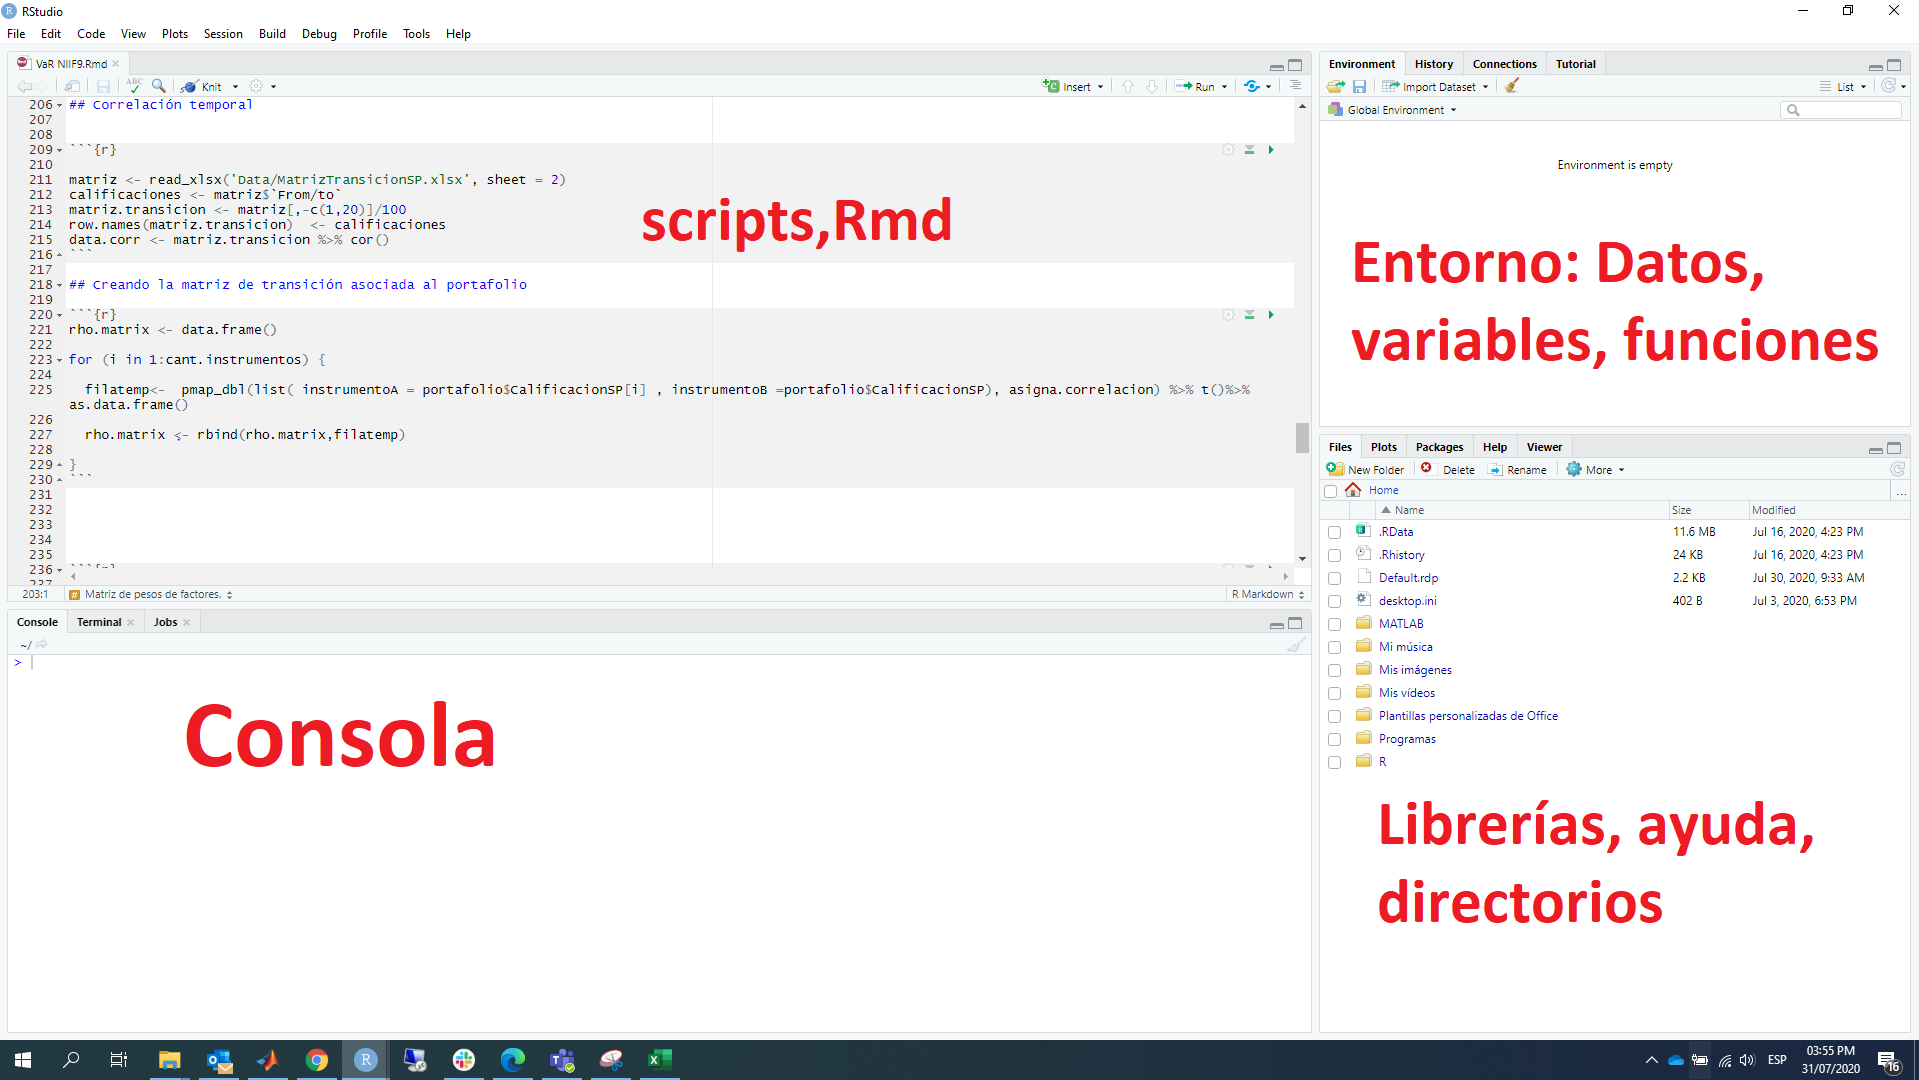
\includegraphics[width=1\linewidth]{images/entornoRStudio} \end{center}

Una vez estamos en RStudio, podemos escribir y ejecutar las órdenes de varias formas:

\begin{itemize}
\tightlist
\item
  Directamente en la consola
\item
  A través de un script (.R)
\item
  Con ficheros Rmarkdown (.Rmd)
\end{itemize}

\hypertarget{consola-de-r}{%
\subsection{\texorpdfstring{\textbf{Consola de R}}{Consola de R}}\label{consola-de-r}}

La consola de RStudio nos permite interactuar con los comandos de R, es decir, ingresamos una instrucción en la consola y esta retornará el resultado de la ejecución de ese comando, aunque esta es una herramienta muy útil no es la mejor opción cuando nuestro código gana complejidad.

En la consola escribimos \textbf{expresiones}, el símbolo ``\textless-'' es el operador de asignación, aunque también se puede utilizar el símbolo ``=.''

\textbf{Asignación de valores.}

\begin{Shaded}
\begin{Highlighting}[]
\NormalTok{x }\OtherTok{\textless{}{-}} \DecValTok{1}  \CommentTok{\# Asignamos el valor 1 a la variable x}

\NormalTok{texto }\OtherTok{\textless{}{-}} \StringTok{"Bienvenidos"}  \CommentTok{\# Asignamos el valor "Bienvenidos" a la variable texto}
\end{Highlighting}
\end{Shaded}

En R el símbolo ``\#'' indica que es un comentario, cualquier cosa que esté a su derecha (incluido el ``\#'') será ignorado a la hora de ejecutar el código. Este es el único símbolo para hacer comentarios en R y además cabe mencionar que R no soporta comentarios en bloques o multilíneas.

\textbf{Evaluación.}

Cuando escribimos una expresión en la consola, podemos imprimir su valor sin una orden explícita.

\begin{Shaded}
\begin{Highlighting}[]
\NormalTok{x }\OtherTok{\textless{}{-}} \DecValTok{13} \CommentTok{\# No imprime nada, solo asigna el valor}
\end{Highlighting}
\end{Shaded}

\begin{Shaded}
\begin{Highlighting}[]
\NormalTok{x }\CommentTok{\# Se imprime el valor}
\end{Highlighting}
\end{Shaded}

\begin{verbatim}
## [1] 13
\end{verbatim}

\begin{Shaded}
\begin{Highlighting}[]
\FunctionTok{print}\NormalTok{(x) }\CommentTok{\# Orden explicita}
\end{Highlighting}
\end{Shaded}

\begin{verbatim}
## [1] 13
\end{verbatim}

\hypertarget{ayuda-en-r}{%
\subsection{\texorpdfstring{\textbf{Ayuda en R}}{Ayuda en R}}\label{ayuda-en-r}}

Al comenzar a trabajar con R necesitaremos información sobre cada instrucción,
función y paquete. Toda la documentación se encuentra integrada en RStudio, para accesar a esta información podemos usar la función \textbf{help()} o el signo de interrogación \textbf{?}, de la siguiente manera

\begin{Shaded}
\begin{Highlighting}[]
\FunctionTok{help}\NormalTok{(}\StringTok{"funcion"}\NormalTok{)}

\NormalTok{?funcion}
\NormalTok{??nombre\_paquete}
\end{Highlighting}
\end{Shaded}

Al ejecutar estas instrucciones la información aparece en la pestaña de \textbf{help}.

\begin{Shaded}
\begin{Highlighting}[]
\FunctionTok{help}\NormalTok{(}\StringTok{"read.table"}\NormalTok{)}

\NormalTok{?read.table}
\end{Highlighting}
\end{Shaded}

\hypertarget{nombres-en-r}{%
\subsection{\texorpdfstring{\textbf{Nombres en R}}{Nombres en R}}\label{nombres-en-r}}

Al igual que la documentación de nuestro código, es importante el nombre que le demos a nuestros objetos (variables, funciones). En \textbf{R} los nombres de los objetos deben comenzar con una letra y solo pueden contener letras, números y los signos : "\emph{" , ``.'' Es bueno que los nombres sean descriptivos, es necesario adoptar una convención, la más común es la del guión bajo (snake\_case) en la que los nombres se escriben en minúscula y separados por } .

\begin{Shaded}
\begin{Highlighting}[]
\NormalTok{yo\_uso\_guion\_bajo  }\DocumentationTok{\#\# snake\_case}

\NormalTok{OtraGenteUsaMayusculas}

\NormalTok{algunas.personas.usan.puntos }\DocumentationTok{\#\# Esto es peculiar de R, ya que en otros lenguajes el punto no se acepta en los nombres}
\DocumentationTok{\#\# ya que tiene otras funciones}

\NormalTok{Y\_algunasPocas.Personas\_RENIEGANdelasconvenciones}
\end{Highlighting}
\end{Shaded}

Generalmente las variables son sustantivos y el nombre de las funciones verbos, se debe procurar que los nombres sean concisos y con significado.

\begin{Shaded}
\begin{Highlighting}[]
\DocumentationTok{\#\# Correcto}

\NormalTok{dia\_uno }\OtherTok{\textless{}{-}} \DecValTok{10}

\DocumentationTok{\#\# Incorrecto}

\NormalTok{primer\_dia\_del\_mes }\OtherTok{\textless{}{-}} \DecValTok{10}
\end{Highlighting}
\end{Shaded}

También se debe evitar utilizar nombres de funciones o variables comunes, esto causa confusión al leer el código.

\begin{Shaded}
\begin{Highlighting}[]
\DocumentationTok{\#\# Incorrecto}

\NormalTok{T }\OtherTok{\textless{}{-}} \ConstantTok{FALSE}
\NormalTok{c }\OtherTok{\textless{}{-}} \DecValTok{10}

\NormalTok{mean }\OtherTok{\textless{}{-}} \ControlFlowTok{function}\NormalTok{(x) \{}
  \FunctionTok{sum}\NormalTok{(x)}
\NormalTok{\}}
\end{Highlighting}
\end{Shaded}

Existen muchas otras buenas prácticas a la hora de escribir código en \textbf{R}, el siguiente link contiene una guía del estilo \emph{tidyverse}.

\url{https://style.tidyverse.org/index.html}

\hypertarget{scripts-de-r}{%
\subsection{\texorpdfstring{\textbf{Scripts de R}}{Scripts de R}}\label{scripts-de-r}}

Trabajar en la consola es muy limitado ya que las instrucciones se tienen que escribir una por una. Lo habitual es trabajar con scripts o ficheros de instrucciones. Estos ficheros tienen extensión \textbf{.R}.

Se puede crear una script con cualquier editor de texto, pero nosotros lo haremos desde RStudio. Para hacer esto, seleccionamos la siguiente ruta de menús: File \textgreater{} New File \textgreater{} R script

\begin{center}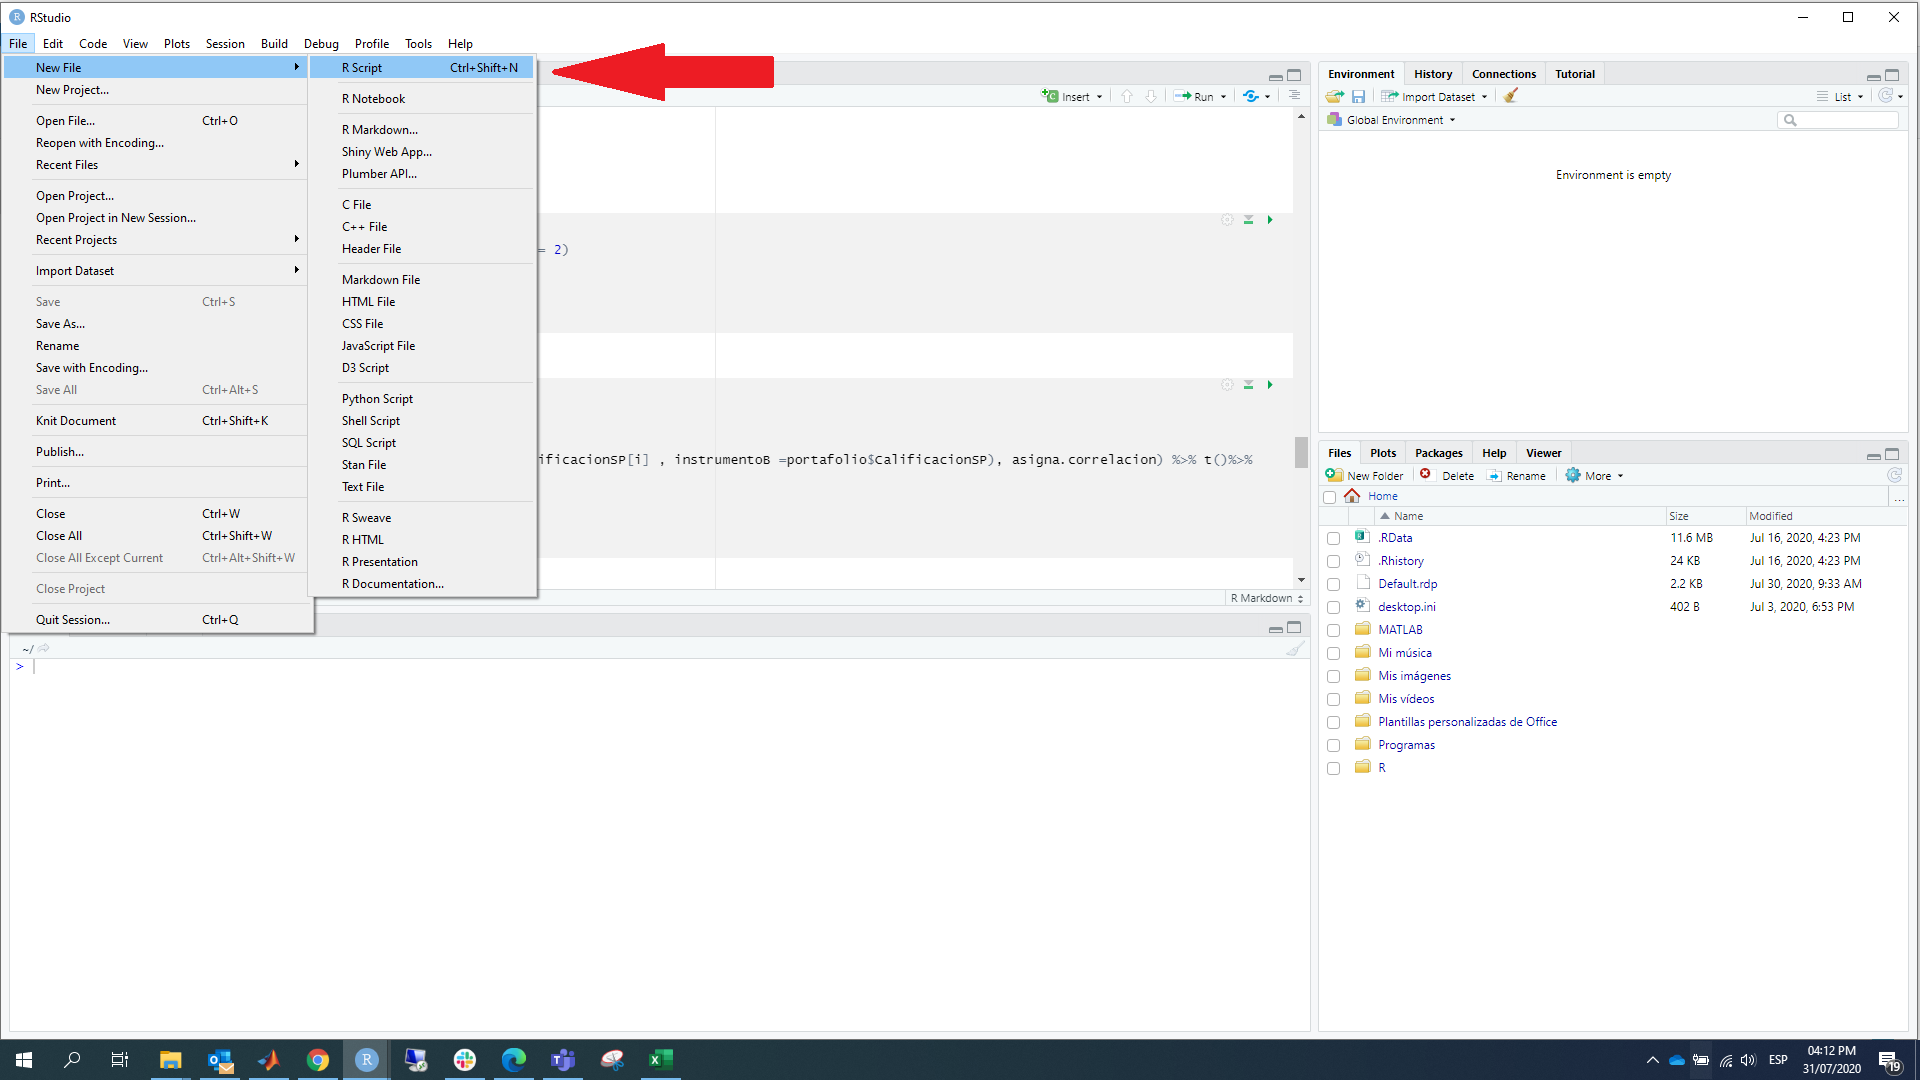
\includegraphics[width=1\linewidth]{images/script} \end{center}

\hypertarget{entorno}{%
\subsection{\texorpdfstring{\textbf{Entorno}}{Entorno}}\label{entorno}}

El panel de entorno esta compuesto de dos pestañas: Environment y History.

En el entorno se irán registrando los objetos que vayamos creando en la sesión de trabajo: datos, variables, funciones. También tenemos la opción de cargar y guardar una sesión de trabajo, importar datos y limpiar los objetos de la sesión. Estas opciones están accesibles a través de las de opciones de la pestaña.

\begin{center}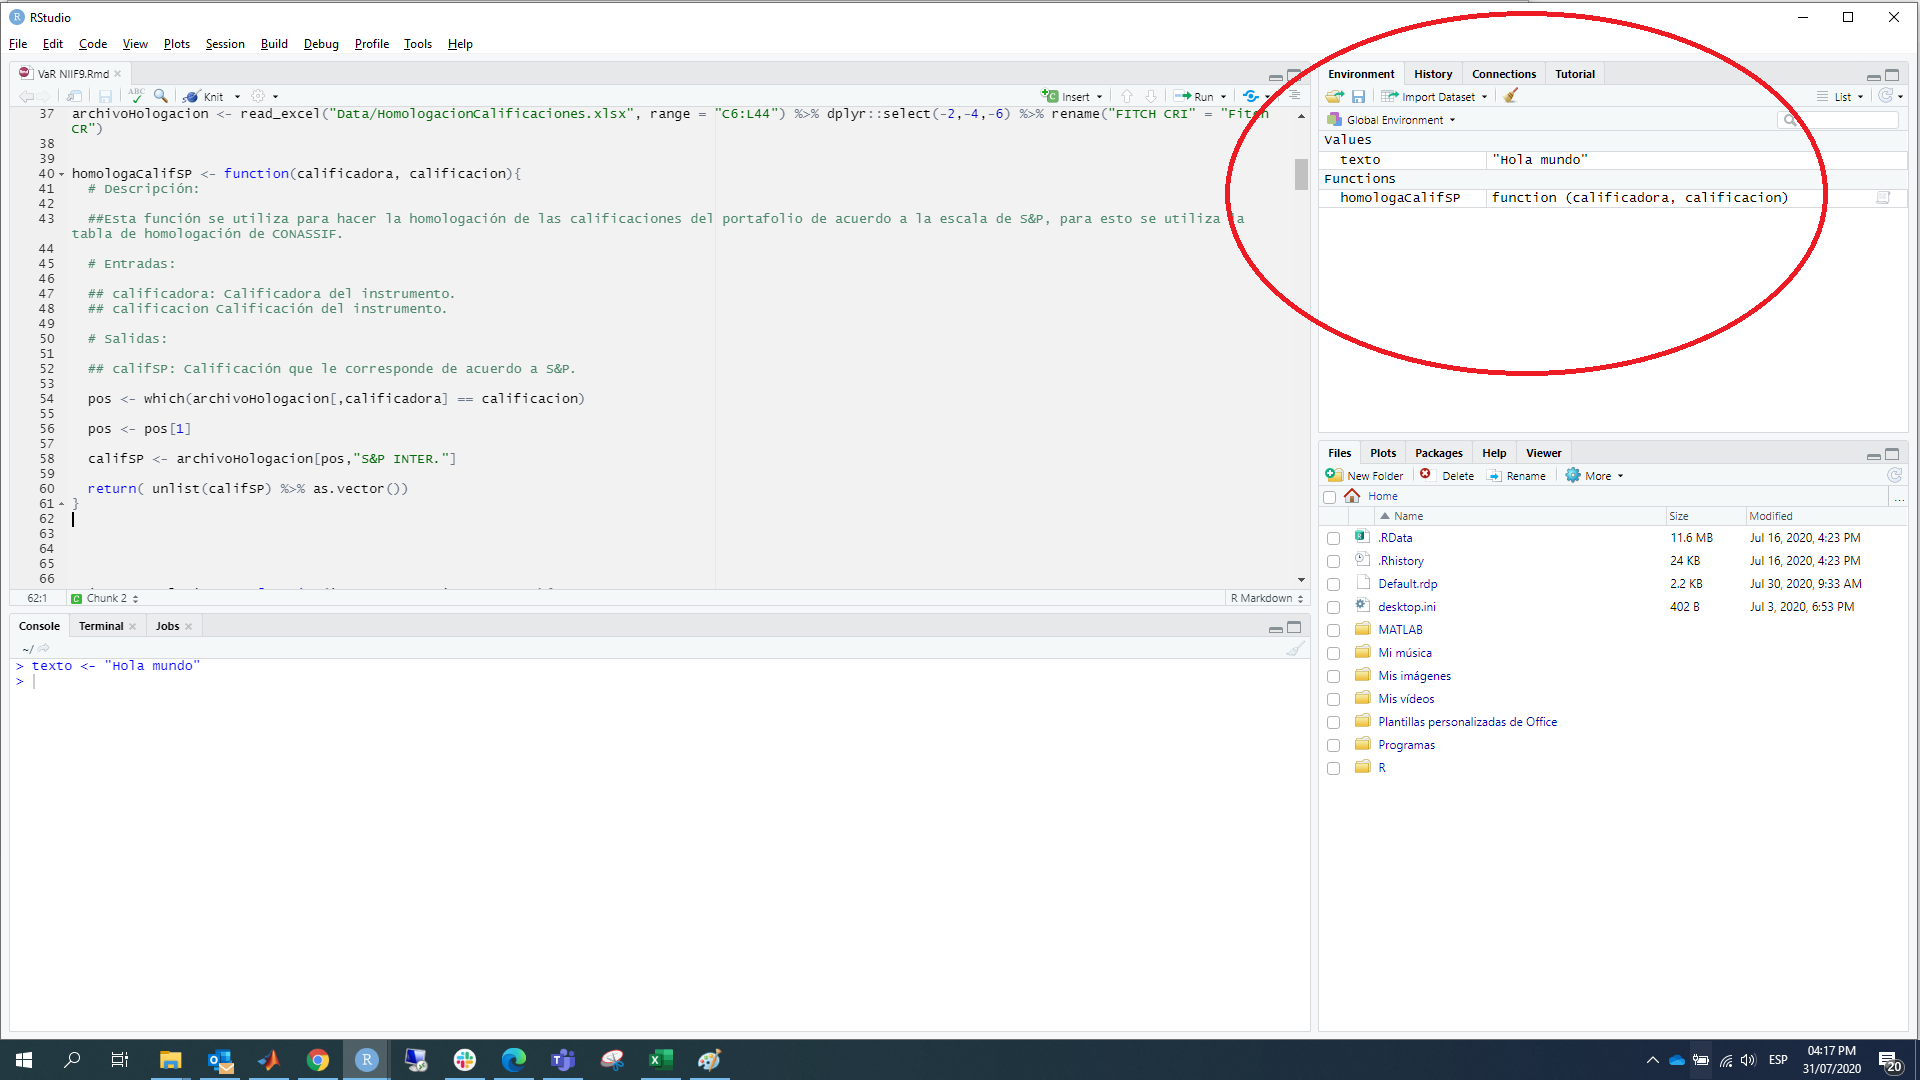
\includegraphics[width=1\linewidth]{images/entorno} \end{center}

\hypertarget{directorio-de-trabajo}{%
\subsection{\texorpdfstring{\textbf{Directorio de trabajo}}{Directorio de trabajo}}\label{directorio-de-trabajo}}

El directorio o carpeta de trabajo es el lugar en la computadora en el que se encuentran los archivos con los que se van a trabajar en R. Este es el lugar donde R buscara archivos para importarlos y al que serán exportados, a menos que indiquemos otra cosa.

Para encontrar cuál es el directorio de trabajo actual se utiliza la función \textbf{getwd()}.

\begin{Shaded}
\begin{Highlighting}[]
\FunctionTok{getwd}\NormalTok{()}
\end{Highlighting}
\end{Shaded}

\begin{verbatim}
## [1] "/Users/tchavarria/Documents/GitHub/programacion-r-basico"
\end{verbatim}

Se mostrará en la consola la ruta del directorio que está usando R.

Se puede cambiar el directorio de trabajo usando la función setwd(), dando como argumento la ruta del directorio que se desea utilizar.

\begin{Shaded}
\begin{Highlighting}[]
\FunctionTok{setwd}\NormalTok{(}\StringTok{"otra\_ruta"}\NormalTok{)}
\end{Highlighting}
\end{Shaded}

\hypertarget{paquetes}{%
\section{\texorpdfstring{\textbf{Paquetes}}{Paquetes}}\label{paquetes}}

Cada paquete es una colección de funciones diseñadas para atender una tarea específica. Por ejemplo, hay paquetes para trabajo visualización, conexiones a bases de datos, minería de datos, interacción con servicios de internet, entre otros.

Estos paquetes se encuentran alojados en CRAN, así que pasan por un control riguroso antes de estar disponibles para su uso generalizado.

Se pueden instalar paquetes usando la función \textbf{install.packages()}, dando como argumento el nombre del paquete que deseamos instalar, entre comillas.

Por ejemplo, para instalar el paquete \textbf{dplyr}, ejecutamos lo siguiente.

\begin{Shaded}
\begin{Highlighting}[]
\FunctionTok{install.packages}\NormalTok{(}\StringTok{"dplyr"}\NormalTok{) }\DocumentationTok{\#\# En general se escribe  install.packages("nombre\_paquete")}
\end{Highlighting}
\end{Shaded}

Después de ejecutar esa instrucción, aparecerán algunos mensajes en la consola mostrando el avance de la instalación

Una vez concluida la instalación de un paquete, para poder utilizar sus funciones debemos ejecutar la función \textbf{library()} con el nombre del paquete que se quiere utilizar.

\begin{Shaded}
\begin{Highlighting}[]
\FunctionTok{library}\NormalTok{(dplyr)   }\DocumentationTok{\#\# En general se escribe  library("nombre\_paquete")}
\end{Highlighting}
\end{Shaded}

\hypertarget{scripts}{%
\section{\texorpdfstring{\textbf{Scripts}}{Scripts}}\label{scripts}}

Los scripts son documentos de texto con la extensión de archivo .R, por ejemplo mi\_script.R.

Estos archivos son iguales a cualquier documentos de texto, pero R los puede leer y ejecutar el código que contienen.

Aunque R permite el uso interactivo, es recomendable guardar el código en un archivo .R, de esta manera se puede utilizar después y compartirlo con otras personas. En general, en proyectos complejos, es posible que sean necesarios múltiples scripts para distintos fines.

Se pueden abrir y ejecutar scripts en R usando la función \textbf{source()}, esta recibe como argumento la ruta del archivo .R en nuestra computadora, entre comillas.

Por ejemplo.

\begin{Shaded}
\begin{Highlighting}[]
\FunctionTok{source}\NormalTok{(}\StringTok{"C:/Proyecto/limpiezaDatos.R"}\NormalTok{)}
\end{Highlighting}
\end{Shaded}

Cuando usamos RStudio y abrimos un script con extensión .R, este programa abre un panel en el que se puede ver su contenido. De este modo se puede ejecutar todo el código que contiene o sólo partes de él.

\hypertarget{shortcuts}{%
\section{\texorpdfstring{\textbf{Shortcuts}}{Shortcuts}}\label{shortcuts}}

\begin{itemize}
\tightlist
\item
  Borrar toda la consola: CTRL + L.
\item
  Ejecutar una línea o lo que se seleccione: CTRL+R
\end{itemize}

\hypertarget{objetos-en-r.}{%
\chapter{\texorpdfstring{\textbf{Objetos en R.}}{Objetos en R.}}\label{objetos-en-r.}}

En R tenemos 5 clases de objeto básicos o atómicos:

\begin{itemize}
\tightlist
\item
  character
\item
  numeric
\item
  integer
\item
  complex
\item
  logical (TRUE/FALSE)
\end{itemize}

\begin{Shaded}
\begin{Highlighting}[]
\NormalTok{tipo.bien }\OtherTok{\textless{}{-}} \StringTok{"Vivienda"}   \DocumentationTok{\#\# character}

\NormalTok{saldo }\OtherTok{\textless{}{-}} \FloatTok{130500.34}        \DocumentationTok{\#\# numeric}

\NormalTok{meses }\OtherTok{\textless{}{-}} \DecValTok{13}               \DocumentationTok{\#\# numeric}

\NormalTok{dias.mora }\OtherTok{\textless{}{-}}\NormalTok{ 10L          }\DocumentationTok{\#\# integer}

\NormalTok{complejo }\OtherTok{\textless{}{-}} \DecValTok{1} \SpecialCharTok{+}\NormalTok{ 3i         }\DocumentationTok{\#\# complex}

\NormalTok{cobro.judicial }\OtherTok{\textless{}{-}} \ConstantTok{TRUE}    \DocumentationTok{\#\# logical}
\end{Highlighting}
\end{Shaded}

\textbf{Números.}

\begin{itemize}
\tightlist
\item
  En R los número en general se tratan como objetos numeric (i.e números reales de doble precisión.)
\item
  Existe el valor \textbf{Inf} que representa infinito y se asocia a operaciones como : 1/0.
\end{itemize}

\begin{Shaded}
\begin{Highlighting}[]
\DecValTok{1} \SpecialCharTok{/} \DecValTok{0}
\end{Highlighting}
\end{Shaded}

\begin{verbatim}
## [1] Inf
\end{verbatim}

\begin{Shaded}
\begin{Highlighting}[]
\SpecialCharTok{{-}}\DecValTok{1} \SpecialCharTok{/} \DecValTok{0}
\end{Highlighting}
\end{Shaded}

\begin{verbatim}
## [1] -Inf
\end{verbatim}

\begin{Shaded}
\begin{Highlighting}[]
\DecValTok{100} \SpecialCharTok{/} \ConstantTok{Inf}
\end{Highlighting}
\end{Shaded}

\begin{verbatim}
## [1] 0
\end{verbatim}

\begin{itemize}
\tightlist
\item
  El valor \textbf{NaN} significa not a number, este se asocia generalmente a datos ausentes pero también a una operación del tipo 0/0 que no está definida.
\end{itemize}

\textbf{Atributos}

Los objetos en R pueden tener los siguientes atributos

\begin{itemize}
\tightlist
\item
  names, dimnames (matrices, data frames)
\item
  dimension (matrices, data frames)
\item
  class
\item
  length
\end{itemize}

más adelante veremos que con detalle el uso de estos.

\hypertarget{operadores}{%
\chapter{\texorpdfstring{\textbf{Operadores}}{Operadores}}\label{operadores}}

\textbf{Operadores aritméticos}

En R tenemos los siguientes operadores aritméticos:

\begin{longtable}[]{@{}rrlll@{}}
\toprule
Operador & Operación & Ejemplo & Resultado &\tabularnewline
\midrule
\endhead
+ & Suma & 3+1 & 4 &\tabularnewline
- & Resta & 4-6 & -2 &\tabularnewline
* & Multiplicación & 4*6 & 24 &\tabularnewline
/ & División & 14/5 & 2.8 &\tabularnewline
\^{} & Potencia & 2\^{}3 & 8 &\tabularnewline
\%\% & División entera & 5\%\%2 & 1 &\tabularnewline
\bottomrule
\end{longtable}

\textbf{Operadores relacionales}

Los operadores relacionales son usados para hacer comparaciones y siempre devuelven como resultado TRUE o FALSE (verdadero o falso, respectivamente).

\begin{longtable}[]{@{}rrlll@{}}
\toprule
Operador & Operación & Ejemplo & Resultado &\tabularnewline
\midrule
\endhead
\textless{} & Menor estricto & 10 \textless{} 3 & FALSE &\tabularnewline
\textless= & Menor o igual & 10 \textless= 3 & FALSE &\tabularnewline
\textgreater{} & Mayor estricto & 10 \textgreater{} 3 & TRUE &\tabularnewline
\textgreater= & Mayor o igual & 10 \textgreater= 3 & TRUE &\tabularnewline
== & Igual & 10 == 3 & FALSE &\tabularnewline
!= & Distinto & 10 != 3 & TRUE &\tabularnewline
\bottomrule
\end{longtable}

\textbf{Operadores lógicos}

Los operadores lógicos son usados para operaciones de álgebra Booleana, es decir, para describir relaciones lógicas, expresadas como verdadero (TRUE) o falso (FALSO).

\begin{longtable}[]{@{}rrl@{}}
\toprule
Operador & Operación &\tabularnewline
\midrule
\endhead
\textbar{} & or &\tabularnewline
\& & and (conjunción) &\tabularnewline
! & negación &\tabularnewline
\bottomrule
\end{longtable}

Los operadores \textbar{} y \& siguen estas reglas:

\begin{itemize}
\tightlist
\item
  \textbar{} devuelve TRUE si alguno de los datos es TRUE
\item
  \& solo devuelve TRUE si ambos datos es TRUE
\item
  \textbar{} solo devuelve FALSE si ambos datos son FALSE
\item
  \& devuelve FALSE si alguno de los datos es FALSE
\end{itemize}

\begin{Shaded}
\begin{Highlighting}[]
\NormalTok{edad }\OtherTok{\textless{}{-}} \DecValTok{16}
\NormalTok{notas }\OtherTok{\textless{}{-}} \DecValTok{83}

\NormalTok{beca1 }\OtherTok{\textless{}{-}}\NormalTok{ (edad }\SpecialCharTok{\textgreater{}} \DecValTok{18} \SpecialCharTok{\&}\NormalTok{ notas }\SpecialCharTok{\textgreater{}} \DecValTok{80}\NormalTok{)}

\NormalTok{beca1}
\end{Highlighting}
\end{Shaded}

\begin{verbatim}
## [1] FALSE
\end{verbatim}

\begin{Shaded}
\begin{Highlighting}[]
\NormalTok{beca2 }\OtherTok{\textless{}{-}}\NormalTok{ (edad }\SpecialCharTok{\textgreater{}} \DecValTok{18} \SpecialCharTok{|}\NormalTok{ notas }\SpecialCharTok{\textgreater{}} \DecValTok{80}\NormalTok{)}

\NormalTok{beca2}
\end{Highlighting}
\end{Shaded}

\begin{verbatim}
## [1] TRUE
\end{verbatim}

\hypertarget{estructuras-de-datos.}{%
\chapter{\texorpdfstring{\textbf{Estructuras de datos.}}{Estructuras de datos.}}\label{estructuras-de-datos.}}

Las estructuras de datos básicas de R se pueden agrupar por su dimensionalidad y según si son homogéneas (todos los elementos son del mismo tipo) o heterogéneas (hay elementos de distintos tipos). En el siguiente cuadro se resumen estas:

\begin{longtable}[]{@{}rrl@{}}
\toprule
Dimensión & Homogéneas & Heterogéneas\tabularnewline
\midrule
\endhead
1d & Vector & Lista\tabularnewline
2d & Matriz & Data Frame\tabularnewline
\bottomrule
\end{longtable}

\hypertarget{vectores}{%
\section{\texorpdfstring{\textbf{Vectores}}{Vectores}}\label{vectores}}

Los vectores en R son fundamentales ya que, es una de las estructuras de datos más utilizada, la propiedad más importante de los vectores, es que \textbf{solo pueden contener objetos de la misma clase}.

Vectores vacíos pueden crearse con la función \textbf{vector()}, por ejemplo:

\begin{Shaded}
\begin{Highlighting}[]
\FunctionTok{vector}\NormalTok{(}\StringTok{"numeric"}\NormalTok{, }\AttributeTok{length =} \DecValTok{10}\NormalTok{) }\DocumentationTok{\#\# Tiene los parámetros clase y longitud.}
\end{Highlighting}
\end{Shaded}

\begin{verbatim}
##  [1] 0 0 0 0 0 0 0 0 0 0
\end{verbatim}

\begin{Shaded}
\begin{Highlighting}[]
\FunctionTok{vector}\NormalTok{(}\StringTok{"character"}\NormalTok{, }\DecValTok{3}\NormalTok{)}
\end{Highlighting}
\end{Shaded}

\begin{verbatim}
## [1] "" "" ""
\end{verbatim}

Sin embargo, la forma más común para crear vectores es utilizando la función \textbf{c()} que hace referencia a la palabra concatenar.

\begin{Shaded}
\begin{Highlighting}[]
\NormalTok{vector.numerico }\OtherTok{\textless{}{-}} \FunctionTok{c}\NormalTok{(}\DecValTok{1}\NormalTok{, }\DecValTok{2}\NormalTok{, }\FloatTok{3.5}\NormalTok{)   }\DocumentationTok{\#\# numeric}

\NormalTok{vector.logical }\OtherTok{\textless{}{-}} \FunctionTok{c}\NormalTok{(}\ConstantTok{TRUE}\NormalTok{, }\ConstantTok{FALSE}\NormalTok{, T, T, F) }\DocumentationTok{\#\# logical}

\NormalTok{vector.char }\OtherTok{\textless{}{-}} \FunctionTok{c}\NormalTok{(}\StringTok{"Azul"}\NormalTok{, }\StringTok{"Blanco"}\NormalTok{, }\StringTok{"Verde"}\NormalTok{) }\DocumentationTok{\#\# character}

\NormalTok{vector.entero }\OtherTok{\textless{}{-}} \DecValTok{1}\SpecialCharTok{:}\DecValTok{13}   \DocumentationTok{\#\# integer}
\end{Highlighting}
\end{Shaded}

\begin{Shaded}
\begin{Highlighting}[]
\NormalTok{vector.numerico}
\end{Highlighting}
\end{Shaded}

\begin{verbatim}
## [1] 1.0 2.0 3.5
\end{verbatim}

\begin{Shaded}
\begin{Highlighting}[]
\NormalTok{vector.logical}
\end{Highlighting}
\end{Shaded}

\begin{verbatim}
## [1]  TRUE FALSE  TRUE  TRUE FALSE
\end{verbatim}

\begin{Shaded}
\begin{Highlighting}[]
\NormalTok{vector.char}
\end{Highlighting}
\end{Shaded}

\begin{verbatim}
## [1] "Azul"   "Blanco" "Verde"
\end{verbatim}

\begin{Shaded}
\begin{Highlighting}[]
\NormalTok{vector.entero}
\end{Highlighting}
\end{Shaded}

\begin{verbatim}
##  [1]  1  2  3  4  5  6  7  8  9 10 11 12 13
\end{verbatim}

\hypertarget{coerciuxf3n}{%
\subsection{\texorpdfstring{\textbf{Coerción}}{Coerción}}\label{coerciuxf3n}}

Como dijimos anteriormente los vectores solo contienen una misma clase de datos, sin embargo, cuando mezclamos diferentes clases ocurre automáticamente un proceso que se llama \textbf{coerción}, esto básicamente transforma todos los elementos del vector a una misma clase.

\begin{Shaded}
\begin{Highlighting}[]
\NormalTok{vector.prueba1 }\OtherTok{\textless{}{-}} \FunctionTok{c}\NormalTok{(}\FloatTok{1.3}\NormalTok{, }\StringTok{"Diego"}\NormalTok{) }\CommentTok{\# character}
\NormalTok{vector.prueba1}
\end{Highlighting}
\end{Shaded}

\begin{verbatim}
## [1] "1.3"   "Diego"
\end{verbatim}

\begin{Shaded}
\begin{Highlighting}[]
\NormalTok{vector.prueba2 }\OtherTok{\textless{}{-}} \FunctionTok{c}\NormalTok{(}\ConstantTok{TRUE}\NormalTok{, }\DecValTok{13}\NormalTok{, }\ConstantTok{FALSE}\NormalTok{) }\CommentTok{\# numeric  \#TRUE =1 , \# FALSE =0}
\NormalTok{vector.prueba2}
\end{Highlighting}
\end{Shaded}

\begin{verbatim}
## [1]  1 13  0
\end{verbatim}

Una función muy útil es \textbf{length} ya que nos devuelve el tamaño de nuestro vector.

\begin{Shaded}
\begin{Highlighting}[]
\FunctionTok{length}\NormalTok{(vector.prueba2)}
\end{Highlighting}
\end{Shaded}

\begin{verbatim}
## [1] 3
\end{verbatim}

\textbf{Reglas de coerción}:

\begin{itemize}
\item
  Valores lógicos se convierten en numéricos: TRUE = 1, FALSE=0.
\item
  El orden de coerción es el siguiente:

  \begin{itemize}
  \tightlist
  \item
    logical -\textgreater{} integer -\textgreater{} numeric -\textgreater{} character
  \end{itemize}
\end{itemize}

Es decir todos los elementos del vector se van a transformar a la clase correspondiente siguiendo el orden anterior.

\begin{Shaded}
\begin{Highlighting}[]
\NormalTok{vector.prueba3 }\OtherTok{\textless{}{-}} \FunctionTok{c}\NormalTok{(}\DecValTok{12}\NormalTok{, }\ConstantTok{TRUE}\NormalTok{, }\StringTok{"Azul"}\NormalTok{)}

\NormalTok{vector.prueba3}
\end{Highlighting}
\end{Shaded}

\begin{verbatim}
## [1] "12"   "TRUE" "Azul"
\end{verbatim}

Esto es lo que hace R de forma automática, sin embargo, podemos realizar la coerción de forma explícita utilizando la función \textbf{as.}*

\begin{Shaded}
\begin{Highlighting}[]
\CommentTok{\# Vector numerico 0,1,2,3,4,5.}
\NormalTok{x }\OtherTok{\textless{}{-}} \DecValTok{0}\SpecialCharTok{:}\DecValTok{5}
\CommentTok{\# Se transforma a clase logical}
\FunctionTok{as.logical}\NormalTok{(x) }\CommentTok{\# 0 es FALSE, y cualquier otro número es TRUE.}
\end{Highlighting}
\end{Shaded}

\begin{verbatim}
## [1] FALSE  TRUE  TRUE  TRUE  TRUE  TRUE
\end{verbatim}

\begin{Shaded}
\begin{Highlighting}[]
\CommentTok{\# Se transforma a clase character}
\FunctionTok{as.character}\NormalTok{(x)}
\end{Highlighting}
\end{Shaded}

\begin{verbatim}
## [1] "0" "1" "2" "3" "4" "5"
\end{verbatim}

\begin{Shaded}
\begin{Highlighting}[]
\NormalTok{x }\OtherTok{\textless{}{-}} \FunctionTok{as.character}\NormalTok{(x)}
\NormalTok{x}
\end{Highlighting}
\end{Shaded}

\begin{verbatim}
## [1] "0" "1" "2" "3" "4" "5"
\end{verbatim}

Al hacer la coerción de forma explícita es común obtener el siguiente warning:

``Nas introduced by coercion''

Esto significa que dentro del vector hay valores que no tiene sentido convertirlos a la clase que queremos, por ejemplo, convertir

\begin{Shaded}
\begin{Highlighting}[]
\NormalTok{y }\OtherTok{\textless{}{-}} \FunctionTok{c}\NormalTok{(}\StringTok{"A"}\NormalTok{, }\StringTok{"B"}\NormalTok{, }\StringTok{"C"}\NormalTok{)}
\FunctionTok{as.numeric}\NormalTok{(y)}
\end{Highlighting}
\end{Shaded}

\begin{verbatim}
## [1] NA NA NA
\end{verbatim}

Tal vez en el ejemplo anterior no tiene mucho sentido, sin embargo puede pasar que haya una variable que debería contener solo números, pero aparece una letra por error.

\begin{Shaded}
\begin{Highlighting}[]
\NormalTok{y }\OtherTok{\textless{}{-}} \FunctionTok{c}\NormalTok{(}\DecValTok{1}\SpecialCharTok{:}\DecValTok{3}\NormalTok{, }\StringTok{"A"}\NormalTok{, }\DecValTok{5}\SpecialCharTok{:}\DecValTok{7}\NormalTok{)}
\NormalTok{y}
\end{Highlighting}
\end{Shaded}

\begin{verbatim}
## [1] "1" "2" "3" "A" "5" "6" "7"
\end{verbatim}

\begin{Shaded}
\begin{Highlighting}[]
\FunctionTok{as.numeric}\NormalTok{(y)}
\end{Highlighting}
\end{Shaded}

\begin{verbatim}
## [1]  1  2  3 NA  5  6  7
\end{verbatim}

\hypertarget{matrices}{%
\section{\texorpdfstring{\textbf{Matrices}}{Matrices}}\label{matrices}}

Las matrices son vectores pero con el atributo de dimensión. Este atributo es un vector de longitud 2 que contiene el número de filas y el número de columnas (nrow,ncol).

En R la función para crear matrices es \textbf{matrix} recibe cuatro parámetros (dos son opcionales)

\begin{itemize}
\tightlist
\item
  data : vector con los valores que contendrá la matriz.
\item
  nrow : cantidad de filas de la matriz.
\item
  ncol : cantidad de columnas de la matriz.
\item
  byrow : si su valor es TRUE la lectura de los datos se realiza por filas sino se realiza por columnas.
\end{itemize}

\begin{Shaded}
\begin{Highlighting}[]
\NormalTok{matriz1 }\OtherTok{\textless{}{-}} \FunctionTok{matrix}\NormalTok{(}\AttributeTok{nrow =} \DecValTok{2}\NormalTok{, }\AttributeTok{ncol =} \DecValTok{3}\NormalTok{) }\CommentTok{\# No le doy los valores entonces coloca NA en todas las entradas.}

\NormalTok{matriz1}
\end{Highlighting}
\end{Shaded}

\begin{verbatim}
##      [,1] [,2] [,3]
## [1,]   NA   NA   NA
## [2,]   NA   NA   NA
\end{verbatim}

Las matrices se construyen por defecto por columnas, empezando por el valor de la entrada \((1,1)\).

\begin{Shaded}
\begin{Highlighting}[]
\NormalTok{matriz1 }\OtherTok{\textless{}{-}} \FunctionTok{matrix}\NormalTok{(}\DecValTok{1}\SpecialCharTok{:}\DecValTok{9}\NormalTok{, }\AttributeTok{nrow =} \DecValTok{3}\NormalTok{, }\AttributeTok{ncol =} \DecValTok{3}\NormalTok{)}
\NormalTok{matriz1}
\end{Highlighting}
\end{Shaded}

\begin{verbatim}
##      [,1] [,2] [,3]
## [1,]    1    4    7
## [2,]    2    5    8
## [3,]    3    6    9
\end{verbatim}

Esta función nos devuelve la cantidad de filas y columnas de nuestra matriz.

\begin{Shaded}
\begin{Highlighting}[]
\NormalTok{dimensiones }\OtherTok{\textless{}{-}} \FunctionTok{dim}\NormalTok{(matriz1)}

\NormalTok{dimensiones}
\end{Highlighting}
\end{Shaded}

\begin{verbatim}
## [1] 3 3
\end{verbatim}

Es muy común utilizar solo uno de estos valores, estos se pueden obtener mediante la siguiente instrucción.

\begin{Shaded}
\begin{Highlighting}[]
\NormalTok{filas }\OtherTok{\textless{}{-}}\NormalTok{  dimensiones[}\DecValTok{1}\NormalTok{]}
\NormalTok{columnas }\OtherTok{\textless{}{-}}\NormalTok{ dimensiones[}\DecValTok{2}\NormalTok{]}

\NormalTok{filas}
\end{Highlighting}
\end{Shaded}

\begin{verbatim}
## [1] 3
\end{verbatim}

\begin{Shaded}
\begin{Highlighting}[]
\NormalTok{columnas}
\end{Highlighting}
\end{Shaded}

\begin{verbatim}
## [1] 3
\end{verbatim}

Sin embargo se puede cambiar a que se construyan por filas asignando el parámetro \textbf{byrow} en TRUE.

\begin{Shaded}
\begin{Highlighting}[]
\NormalTok{matriz2 }\OtherTok{\textless{}{-}} \FunctionTok{matrix}\NormalTok{(}\DecValTok{1}\SpecialCharTok{:}\DecValTok{9}\NormalTok{, }\AttributeTok{nrow =} \DecValTok{3}\NormalTok{, }\AttributeTok{ncol =} \DecValTok{3}\NormalTok{, }\AttributeTok{byrow =}\NormalTok{ T)}
\NormalTok{matriz2}
\end{Highlighting}
\end{Shaded}

\begin{verbatim}
##      [,1] [,2] [,3]
## [1,]    1    2    3
## [2,]    4    5    6
## [3,]    7    8    9
\end{verbatim}

Un par de funciones útiles a la hora de crear matrices o conjuntos de datos son \textbf{rbind} y \textbf{cbind} que permiten concatenar objetos en forma de filas y columnas respectivamente.

\begin{Shaded}
\begin{Highlighting}[]
\NormalTok{x }\OtherTok{\textless{}{-}} \DecValTok{1}\SpecialCharTok{:}\DecValTok{5}

\NormalTok{y }\OtherTok{\textless{}{-}} \DecValTok{11}\SpecialCharTok{:}\DecValTok{15}

\FunctionTok{rbind}\NormalTok{(x, y)}
\end{Highlighting}
\end{Shaded}

\begin{verbatim}
##   [,1] [,2] [,3] [,4] [,5]
## x    1    2    3    4    5
## y   11   12   13   14   15
\end{verbatim}

\begin{Shaded}
\begin{Highlighting}[]
\FunctionTok{cbind}\NormalTok{(x, y)}
\end{Highlighting}
\end{Shaded}

\begin{verbatim}
##      x  y
## [1,] 1 11
## [2,] 2 12
## [3,] 3 13
## [4,] 4 14
## [5,] 5 15
\end{verbatim}

\hypertarget{data-frames}{%
\section{\texorpdfstring{\textbf{Data Frames}}{Data Frames}}\label{data-frames}}

Los data frames constituyen la manera más eficiente mediante la cual R puede analizar un conjunto de datos estadísticos.

Habitualmente se configuran de tal manera que \textbf{cada fila se refiere a un individuo o unidad estadística, mientras que cada columna hace referencia a una variable estadística}, esa configuración hace que visualmente un data frame parezca una matriz. Sin embargo, como objetos de R, son cosas distintas.

\begin{itemize}
\item
  Los data frames tienen los atributos \textbf{row.names} y \textbf{col.names}.
\item
  Usualmente se crean leyendo datos con las funciones \textbf{read.table()} y \textbf{read.csv()}, pero también podemos utilizar la función \textbf{data.frame()}.
\item
  Se pueden convertir a matrices utilizando la función \textbf{data.matrix()} o \textbf{as.matrix()}.
\end{itemize}

\begin{Shaded}
\begin{Highlighting}[]
\CommentTok{\# Creamos las variables de nuestro data frame.}

\NormalTok{emisor }\OtherTok{\textless{}{-}} \FunctionTok{c}\NormalTok{(}\StringTok{"BL"}\NormalTok{, }\StringTok{"BARCL"}\NormalTok{, }\StringTok{"CSGF"}\NormalTok{, }\StringTok{"CVS"}\NormalTok{, }\StringTok{"DBK"}\NormalTok{, }\StringTok{"G"}\NormalTok{, }\StringTok{"NOMUR"}\NormalTok{, }\StringTok{"USTES"}\NormalTok{, }\StringTok{"BNSFI"}\NormalTok{)}

\NormalTok{monto.facial }\OtherTok{\textless{}{-}} \FunctionTok{c}\NormalTok{(}\DecValTok{5000000}\NormalTok{, }\DecValTok{2500000}\NormalTok{, }\DecValTok{10000000}\NormalTok{, }\DecValTok{40000000}\NormalTok{, }\DecValTok{5000000}\NormalTok{, }\DecValTok{40000000}\NormalTok{, }\DecValTok{10000000}\NormalTok{, }\DecValTok{5600000}\NormalTok{, }\DecValTok{50000000}\NormalTok{)}

\NormalTok{categoria }\OtherTok{\textless{}{-}} \FunctionTok{c}\NormalTok{(}\StringTok{"COSTO AMORTIZADO"}\NormalTok{, }\StringTok{"COSTO AMORTIZADO"}\NormalTok{, }\StringTok{"COSTO AMORTIZADO"}\NormalTok{, }\StringTok{"VR CON CAMBIO EN ORI"}\NormalTok{, }\StringTok{"COSTO AMORTIZADO"}\NormalTok{, }\StringTok{"VR CON CAMBIO EN P/G"}\NormalTok{, }\StringTok{"COSTO AMORTIZADO"}\NormalTok{, }\StringTok{"COSTO AMORTIZADO"}\NormalTok{, }\StringTok{"COSTO AMORTIZADO"}\NormalTok{)}

\NormalTok{calificacion.SP }\OtherTok{\textless{}{-}} \FunctionTok{c}\NormalTok{(}\StringTok{"BBB+"}\NormalTok{, }\StringTok{"AA+"}\NormalTok{, }\StringTok{"B+"}\NormalTok{, }\StringTok{"B+"}\NormalTok{, }\StringTok{"B"}\NormalTok{, }\StringTok{"B"}\NormalTok{, }\StringTok{"A+"}\NormalTok{, }\StringTok{"BB{-}"}\NormalTok{, }\StringTok{"BB"}\NormalTok{)}

\NormalTok{isin }\OtherTok{\textless{}{-}} \FunctionTok{c}\NormalTok{(}\StringTok{"US06738EAL92"}\NormalTok{, }\StringTok{"US225433AH43"}\NormalTok{, }\StringTok{"US126650CK42"}\NormalTok{, }\StringTok{"XS2127535131"}\NormalTok{, }\StringTok{"CRG0000B82H3"}\NormalTok{, }\StringTok{"US404280BJ78"}\NormalTok{, }\StringTok{"0NRBNCR00465"}\NormalTok{, }\StringTok{"US9127962Z13"}\NormalTok{, }\StringTok{"US9128283G32"}\NormalTok{)}


\CommentTok{\# Creamos el data frame.}

\NormalTok{portafolio }\OtherTok{\textless{}{-}} \FunctionTok{data.frame}\NormalTok{(}\AttributeTok{ISIN =}\NormalTok{ isin, }\AttributeTok{Emisor =}\NormalTok{ emisor, }\AttributeTok{Monto.Facial =}\NormalTok{ monto.facial, }\AttributeTok{Categoria\_NIIF =}\NormalTok{ categoria, }\AttributeTok{Calificacion =}\NormalTok{ calificacion.SP)}


\NormalTok{portafolio}
\end{Highlighting}
\end{Shaded}

\begin{verbatim}
##           ISIN Emisor Monto.Facial       Categoria_NIIF Calificacion
## 1 US06738EAL92     BL      5.0e+06     COSTO AMORTIZADO         BBB+
## 2 US225433AH43  BARCL      2.5e+06     COSTO AMORTIZADO          AA+
## 3 US126650CK42   CSGF      1.0e+07     COSTO AMORTIZADO           B+
## 4 XS2127535131    CVS      4.0e+07 VR CON CAMBIO EN ORI           B+
## 5 CRG0000B82H3    DBK      5.0e+06     COSTO AMORTIZADO            B
## 6 US404280BJ78      G      4.0e+07 VR CON CAMBIO EN P/G            B
## 7 0NRBNCR00465  NOMUR      1.0e+07     COSTO AMORTIZADO           A+
## 8 US9127962Z13  USTES      5.6e+06     COSTO AMORTIZADO          BB-
## 9 US9128283G32  BNSFI      5.0e+07     COSTO AMORTIZADO           BB
\end{verbatim}

\begin{Shaded}
\begin{Highlighting}[]
\FunctionTok{dim}\NormalTok{(portafolio)}
\end{Highlighting}
\end{Shaded}

\begin{verbatim}
## [1] 9 5
\end{verbatim}

\hypertarget{listas}{%
\section{\texorpdfstring{\textbf{Listas}}{Listas}}\label{listas}}

Con los data frames vimos que se pueden guardar diferentes tipos de datos en columnas.

Ahora queremos ir un poco más allá y guardar diferentes objetos en una misma estructura de datos.

Las listas permiten agrupar o contener cosas como dataframes, matrices y vectores en una misma variable.

Para crear una lista podemos utilizar la función \textbf{list()}, por ejemplo

\begin{Shaded}
\begin{Highlighting}[]
\NormalTok{lista1 }\OtherTok{\textless{}{-}} \FunctionTok{list}\NormalTok{(}\DecValTok{1}\NormalTok{, }\StringTok{"A"}\NormalTok{, }\ConstantTok{TRUE}\NormalTok{) }\CommentTok{\# integer, character, logical}
\NormalTok{lista1}
\end{Highlighting}
\end{Shaded}

\begin{verbatim}
## [[1]]
## [1] 1
## 
## [[2]]
## [1] "A"
## 
## [[3]]
## [1] TRUE
\end{verbatim}

\begin{Shaded}
\begin{Highlighting}[]
\NormalTok{mi\_vector }\OtherTok{\textless{}{-}} \DecValTok{1}\SpecialCharTok{:}\DecValTok{10}
\NormalTok{mi\_matriz }\OtherTok{\textless{}{-}} \FunctionTok{matrix}\NormalTok{(}\DecValTok{1}\SpecialCharTok{:}\DecValTok{4}\NormalTok{, }\AttributeTok{nrow =} \DecValTok{2}\NormalTok{)}

\NormalTok{mi\_dataframe }\OtherTok{\textless{}{-}} \FunctionTok{data.frame}\NormalTok{(}\StringTok{"numeros"} \OtherTok{=} \DecValTok{1}\SpecialCharTok{:}\DecValTok{3}\NormalTok{, }\StringTok{"letras"} \OtherTok{=} \FunctionTok{c}\NormalTok{(}\StringTok{"a"}\NormalTok{, }\StringTok{"b"}\NormalTok{, }\StringTok{"c"}\NormalTok{))}

\NormalTok{mi\_lista }\OtherTok{\textless{}{-}} \FunctionTok{list}\NormalTok{(}\StringTok{"un\_vector"} \OtherTok{=}\NormalTok{ mi\_vector, }\StringTok{"una\_matriz"} \OtherTok{=}\NormalTok{ mi\_matriz, }\StringTok{"un\_df"} \OtherTok{=}\NormalTok{ mi\_dataframe)}

\NormalTok{mi\_lista}
\end{Highlighting}
\end{Shaded}

\begin{verbatim}
## $un_vector
##  [1]  1  2  3  4  5  6  7  8  9 10
## 
## $una_matriz
##      [,1] [,2]
## [1,]    1    3
## [2,]    2    4
## 
## $un_df
##   numeros letras
## 1       1      a
## 2       2      b
## 3       3      c
\end{verbatim}

Cuando creamos listas lo más común es nombrar cada una de las entradas para luego poder extraer esos datos con el signo ``\$.''

\begin{Shaded}
\begin{Highlighting}[]
\NormalTok{lista\_clientes }\OtherTok{\textless{}{-}} \FunctionTok{list}\NormalTok{(}\AttributeTok{saldo =} \FunctionTok{runif}\NormalTok{(}\DecValTok{3}\NormalTok{, }\AttributeTok{min =} \DecValTok{1000}\NormalTok{, }\AttributeTok{max =} \DecValTok{2000}\NormalTok{), }\AttributeTok{nombres =} \FunctionTok{c}\NormalTok{(}\StringTok{"Juan"}\NormalTok{, }\StringTok{"Luis"}\NormalTok{, }\StringTok{"Carlos"}\NormalTok{), }\AttributeTok{tarjeta.credito =} \FunctionTok{c}\NormalTok{(T, T, F))}


\NormalTok{lista\_clientes}
\end{Highlighting}
\end{Shaded}

\begin{verbatim}
## $saldo
## [1] 1120.933 1558.749 1723.265
## 
## $nombres
## [1] "Juan"   "Luis"   "Carlos"
## 
## $tarjeta.credito
## [1]  TRUE  TRUE FALSE
\end{verbatim}

\begin{Shaded}
\begin{Highlighting}[]
\CommentTok{\# runif(cantidad, min, max) genera números aleatorios.}
\end{Highlighting}
\end{Shaded}

\begin{Shaded}
\begin{Highlighting}[]
\NormalTok{lista\_clientes}\SpecialCharTok{$}\NormalTok{saldo}
\end{Highlighting}
\end{Shaded}

\begin{verbatim}
## [1] 1120.933 1558.749 1723.265
\end{verbatim}

Otro ejemplo:

\begin{Shaded}
\begin{Highlighting}[]
\NormalTok{datos.lucas }\OtherTok{\textless{}{-}} \FunctionTok{list}\NormalTok{(}\AttributeTok{Nombre =} \StringTok{"Lucas"}\NormalTok{, }\AttributeTok{Edad =} \DecValTok{33}\NormalTok{, }\AttributeTok{Tarjeta.Credito =} \ConstantTok{FALSE}\NormalTok{)}

\NormalTok{datos.lucas}
\end{Highlighting}
\end{Shaded}

\begin{verbatim}
## $Nombre
## [1] "Lucas"
## 
## $Edad
## [1] 33
## 
## $Tarjeta.Credito
## [1] FALSE
\end{verbatim}

Una ventaja del objeto lista es que podemos accesar a cada uno de sus argumentos mediante el símbolo ``\$,'' por ejemplo si quisieramos ver su Edad y luego si posee tarjeta de crédito o no, podemos escribir

\begin{Shaded}
\begin{Highlighting}[]
\NormalTok{datos.lucas}\SpecialCharTok{$}\NormalTok{Edad}
\end{Highlighting}
\end{Shaded}

\begin{verbatim}
## [1] 33
\end{verbatim}

\begin{Shaded}
\begin{Highlighting}[]
\NormalTok{datos.lucas}\SpecialCharTok{$}\NormalTok{Tarjeta.Credito}
\end{Highlighting}
\end{Shaded}

\begin{verbatim}
## [1] FALSE
\end{verbatim}

\hypertarget{factores}{%
\section{\texorpdfstring{\textbf{Factores}}{Factores}}\label{factores}}

Esta clase de datos se utiliza para representar datos categóricos. Estos pueden ser ordenados y sin orden. Podemos pensar en los factores como un vector de enteros, donde cada número representa una categoría.

\begin{itemize}
\tightlist
\item
  Los factores tienen un tratamiento especial en las funciones de modelación como lm() y glm(). (Regresiones lineales)
\item
  Es mejor utilizar factores que utilizar enteros, por ejemplo tener la variable Estado civil, con los valores ``Casado,'' ``Soltero'' es mejor que utilizar los valores 1 y 2.
\end{itemize}

La función para crear variables categóricas es \textbf{factor()}

\begin{Shaded}
\begin{Highlighting}[]
\NormalTok{estado.deuda }\OtherTok{\textless{}{-}} \FunctionTok{factor}\NormalTok{(}\FunctionTok{c}\NormalTok{(}\StringTok{"NORMAL"}\NormalTok{, }\StringTok{"NORMAL"}\NormalTok{, }\StringTok{"VENCIDA"}\NormalTok{, }\StringTok{"COBRO JUDICIAL"}\NormalTok{, }\StringTok{"VENCIDA"}\NormalTok{))}
\NormalTok{estado.deuda}
\end{Highlighting}
\end{Shaded}

\begin{verbatim}
## [1] NORMAL         NORMAL         VENCIDA        COBRO JUDICIAL VENCIDA       
## Levels: COBRO JUDICIAL NORMAL VENCIDA
\end{verbatim}

Como podemos ver, al imprimir nuestra variable categórica tenemos tres niveles : COBRO JUDICIAL NORMAL VENCIDA. Estos representan las categorías en nuestra variable. R automáticamente hace está asignación por orden alfabético, si queremos definir nosotros el orden, podemos hacerlo utilizando el parámetro \textbf{levels}.

\begin{Shaded}
\begin{Highlighting}[]
\NormalTok{estado.deuda }\OtherTok{\textless{}{-}} \FunctionTok{factor}\NormalTok{(}\FunctionTok{c}\NormalTok{(}\StringTok{"NORMAL"}\NormalTok{, }\StringTok{"NORMAL"}\NormalTok{, }\StringTok{"VENCIDA"}\NormalTok{, }\StringTok{"COBRO JUDICIAL"}\NormalTok{, }\StringTok{"VENCIDA"}\NormalTok{), }\AttributeTok{levels =} \FunctionTok{c}\NormalTok{(}\StringTok{"NORMAL"}\NormalTok{, }\StringTok{"VENCIDA"}\NormalTok{, }\StringTok{"COBRO JUDICIAL"}\NormalTok{))}

\NormalTok{estado.deuda}
\end{Highlighting}
\end{Shaded}

\begin{verbatim}
## [1] NORMAL         NORMAL         VENCIDA        COBRO JUDICIAL VENCIDA       
## Levels: NORMAL VENCIDA COBRO JUDICIAL
\end{verbatim}

Una forma de saber cuantos individuos hay en cada categoría es mediante la función \textbf{table()}.

\begin{Shaded}
\begin{Highlighting}[]
\FunctionTok{table}\NormalTok{(estado.deuda)}
\end{Highlighting}
\end{Shaded}

\begin{verbatim}
## estado.deuda
##         NORMAL        VENCIDA COBRO JUDICIAL 
##              2              2              1
\end{verbatim}

\hypertarget{valores-ausentes}{%
\section{\texorpdfstring{\textbf{Valores ausentes}}{Valores ausentes}}\label{valores-ausentes}}

Los valores ausentes se denotan por \textbf{NA} (not avaiable) o \textbf{NaN}(not a number), las siguientes funciones se utilizan para verificar y encontrar valores ausentes.

\begin{enumerate}
\def\labelenumi{\arabic{enumi}.}
\item
  \textbf{is.na()}: Se utiliza para verificar y encontrar los valores \textbf{NA} en un objeto.
\item
  \textbf{is.nan()}: Se utiliza para verificar y encontrar los valores \textbf{NaN} en un objeto.
\item
  Un valor \textbf{NaN} es un \textbf{NA} pero la otra dirección no es cierta.
\end{enumerate}

\begin{Shaded}
\begin{Highlighting}[]
\DocumentationTok{\#\# Creamos un vector que contenga un NA}
\NormalTok{x }\OtherTok{\textless{}{-}} \FunctionTok{c}\NormalTok{(}\DecValTok{1}\NormalTok{, }\DecValTok{3}\NormalTok{, }\ConstantTok{NA}\NormalTok{, }\DecValTok{10}\NormalTok{, }\DecValTok{3}\NormalTok{)}

\DocumentationTok{\#\# Retorna un vector de la misma longitud de x, con TRUE donde hay un NA y FALSE donde no.}
\FunctionTok{is.na}\NormalTok{(x)}
\end{Highlighting}
\end{Shaded}

\begin{verbatim}
## [1] FALSE FALSE  TRUE FALSE FALSE
\end{verbatim}

\begin{Shaded}
\begin{Highlighting}[]
\DocumentationTok{\#\# Creamos un vector que contenga un NA y NaN.}
\NormalTok{x }\OtherTok{\textless{}{-}} \FunctionTok{c}\NormalTok{(}\DecValTok{1}\NormalTok{, }\DecValTok{3}\NormalTok{, }\ConstantTok{NA}\NormalTok{, }\DecValTok{10}\NormalTok{, }\DecValTok{3}\NormalTok{, }\ConstantTok{NaN}\NormalTok{)}

\DocumentationTok{\#\# Retorna un vector de la misma longitud de x, con TRUE donde hay un NA y FALSE donde no.}
\FunctionTok{is.na}\NormalTok{(x)}
\end{Highlighting}
\end{Shaded}

\begin{verbatim}
## [1] FALSE FALSE  TRUE FALSE FALSE  TRUE
\end{verbatim}

\begin{Shaded}
\begin{Highlighting}[]
\DocumentationTok{\#\# Retorna un vector de la misma longitud de x, con TRUE donde hay un NA y FALSE donde no.}
\FunctionTok{is.nan}\NormalTok{(x)}
\end{Highlighting}
\end{Shaded}

\begin{verbatim}
## [1] FALSE FALSE FALSE FALSE FALSE  TRUE
\end{verbatim}

con el ejemplo anterior se puede verificar el punto \textbf{3.}.

\hypertarget{subsetting}{%
\chapter{\texorpdfstring{\textbf{Subsetting}}{Subsetting}}\label{subsetting}}

Vamos a ver como podemos obtener subconjuntos de nuestros datos, existen tres tipos de operaciones para extraer subconjuntos de datos en R:

\begin{itemize}
\tightlist
\item
  \([ ]\): Siempre retorna un objeto de la misma clase que el original.
\item
  \([[ ]]\): Se utiliza para extraer elementos de una lista o un data frame, mediante índices lógicos o numéricos. No necesariamente retorna una lista o data frame.
\item
  \$: Se utiliza para extraer elementos de una lista por su nombre.
\end{itemize}

\hypertarget{subsetting-vectores}{%
\section{\texorpdfstring{\textbf{Subsetting vectores}}{Subsetting vectores}}\label{subsetting-vectores}}

Índices numéricos:

\begin{Shaded}
\begin{Highlighting}[]
\NormalTok{x }\OtherTok{\textless{}{-}} \FunctionTok{c}\NormalTok{(}\StringTok{"A"}\NormalTok{, }\StringTok{"BB+"}\NormalTok{, }\StringTok{"CCC"}\NormalTok{, }\StringTok{"AA+"}\NormalTok{, }\StringTok{"B"}\NormalTok{, }\StringTok{"B+"}\NormalTok{)}

\NormalTok{x[}\DecValTok{1}\NormalTok{]}
\end{Highlighting}
\end{Shaded}

\begin{verbatim}
## [1] "A"
\end{verbatim}

\begin{Shaded}
\begin{Highlighting}[]
\NormalTok{x[}\DecValTok{3}\NormalTok{]}
\end{Highlighting}
\end{Shaded}

\begin{verbatim}
## [1] "CCC"
\end{verbatim}

\begin{Shaded}
\begin{Highlighting}[]
\NormalTok{x[}\DecValTok{1}\SpecialCharTok{:}\DecValTok{3}\NormalTok{]}
\end{Highlighting}
\end{Shaded}

\begin{verbatim}
## [1] "A"   "BB+" "CCC"
\end{verbatim}

Algo peculiar y útil en R es que podemos obtener elementos, seleccionando los que \textbf{no} queremos

\begin{Shaded}
\begin{Highlighting}[]
\NormalTok{x[}\SpecialCharTok{{-}}\DecValTok{1}\NormalTok{]  }\DocumentationTok{\#\# Todos excepto el primer elemento}
\end{Highlighting}
\end{Shaded}

\begin{verbatim}
## [1] "BB+" "CCC" "AA+" "B"   "B+"
\end{verbatim}

\begin{Shaded}
\begin{Highlighting}[]
\NormalTok{x[}\SpecialCharTok{{-}}\FunctionTok{c}\NormalTok{(}\DecValTok{1}\NormalTok{, }\DecValTok{3}\NormalTok{, }\DecValTok{5}\NormalTok{)] }\DocumentationTok{\#\# Todos excepto los elementos e la posición 1,3,5.}
\end{Highlighting}
\end{Shaded}

\begin{verbatim}
## [1] "BB+" "AA+" "B+"
\end{verbatim}

Índices lógicos.

\begin{Shaded}
\begin{Highlighting}[]
\CommentTok{\# Vector de enteros del 1 al 10.}
\NormalTok{y }\OtherTok{\textless{}{-}} \FunctionTok{sample}\NormalTok{(}\DecValTok{30}\NormalTok{, }\DecValTok{10}\NormalTok{)}
\CommentTok{\# sample(x,n) retorna n números aleatorios sin repeticiones menores o iguales a x.}
\NormalTok{y}
\end{Highlighting}
\end{Shaded}

\begin{verbatim}
##  [1] 18 30 21 22  9 27 29 20 10 26
\end{verbatim}

\begin{Shaded}
\begin{Highlighting}[]
\CommentTok{\# Retorna un vector con los valores mayores que 4.}
\NormalTok{y[y }\SpecialCharTok{\textgreater{}} \DecValTok{10}\NormalTok{]}
\end{Highlighting}
\end{Shaded}

\begin{verbatim}
## [1] 18 30 21 22 27 29 20 26
\end{verbatim}

Esto también es válido pero es más lardo de escribir.

\begin{Shaded}
\begin{Highlighting}[]
\CommentTok{\# Guardamos un índice lógico que nos devuelve TRUE en las posiciones de y que hay elementos mayores a 4.}
\NormalTok{index }\OtherTok{\textless{}{-}}\NormalTok{ y }\SpecialCharTok{\textgreater{}} \DecValTok{20}
\NormalTok{index}
\end{Highlighting}
\end{Shaded}

\begin{verbatim}
##  [1] FALSE  TRUE  TRUE  TRUE FALSE  TRUE  TRUE FALSE FALSE  TRUE
\end{verbatim}

\begin{Shaded}
\begin{Highlighting}[]
\CommentTok{\# Extraemos los elementos utilizando el índice lógico.}
\NormalTok{y[index]}
\end{Highlighting}
\end{Shaded}

\begin{verbatim}
## [1] 30 21 22 27 29 26
\end{verbatim}

\hypertarget{subsetting-listas}{%
\section{\texorpdfstring{\textbf{Subsetting listas}}{Subsetting listas}}\label{subsetting-listas}}

Para acceder a elementos de las listas podemos usar \textbf{\$} o doble corchete \textbf{{[}{[} {]}{]}}, ambos realizan la misma operación in embargo una usa índice y el otro el nombre del elemento.

\begin{Shaded}
\begin{Highlighting}[]
\NormalTok{datos.cliente }\OtherTok{\textless{}{-}} \FunctionTok{list}\NormalTok{(}\AttributeTok{Nombre =} \FunctionTok{c}\NormalTok{(}\StringTok{"Lucas"}\NormalTok{, }\StringTok{"Luis"}\NormalTok{, }\StringTok{"Diego"}\NormalTok{), }\AttributeTok{Edad =} \FunctionTok{c}\NormalTok{(}\DecValTok{33}\NormalTok{, }\DecValTok{50}\NormalTok{, }\DecValTok{20}\NormalTok{), }\AttributeTok{Tarjeta.Credito =} \FunctionTok{c}\NormalTok{(T, F, T))}

\NormalTok{datos.cliente}
\end{Highlighting}
\end{Shaded}

\begin{verbatim}
## $Nombre
## [1] "Lucas" "Luis"  "Diego"
## 
## $Edad
## [1] 33 50 20
## 
## $Tarjeta.Credito
## [1]  TRUE FALSE  TRUE
\end{verbatim}

\begin{Shaded}
\begin{Highlighting}[]
\NormalTok{datos.cliente}\SpecialCharTok{$}\NormalTok{Nombre}
\end{Highlighting}
\end{Shaded}

\begin{verbatim}
## [1] "Lucas" "Luis"  "Diego"
\end{verbatim}

\begin{Shaded}
\begin{Highlighting}[]
\NormalTok{datos.cliente}\SpecialCharTok{$}\NormalTok{Edad}
\end{Highlighting}
\end{Shaded}

\begin{verbatim}
## [1] 33 50 20
\end{verbatim}

\begin{Shaded}
\begin{Highlighting}[]
\NormalTok{datos.cliente}\SpecialCharTok{$}\NormalTok{Tarjeta.Credito}
\end{Highlighting}
\end{Shaded}

\begin{verbatim}
## [1]  TRUE FALSE  TRUE
\end{verbatim}

\begin{Shaded}
\begin{Highlighting}[]
\NormalTok{datos.cliente[[}\DecValTok{1}\NormalTok{]]}
\end{Highlighting}
\end{Shaded}

\begin{verbatim}
## [1] "Lucas" "Luis"  "Diego"
\end{verbatim}

\begin{Shaded}
\begin{Highlighting}[]
\NormalTok{datos.cliente[[}\DecValTok{2}\NormalTok{]]}
\end{Highlighting}
\end{Shaded}

\begin{verbatim}
## [1] 33 50 20
\end{verbatim}

Si queremos el valor i del elemento j escribimos \[lista[[j]][i]\]

\begin{Shaded}
\begin{Highlighting}[]
\NormalTok{datos.cliente[[}\DecValTok{3}\NormalTok{]][}\DecValTok{1}\NormalTok{] }\DocumentationTok{\#\# Valor 1 del elemento 3.}
\end{Highlighting}
\end{Shaded}

\begin{verbatim}
## [1] TRUE
\end{verbatim}

\hypertarget{subsetting-matrices}{%
\section{\texorpdfstring{\textbf{Subsetting matrices}}{Subsetting matrices}}\label{subsetting-matrices}}

Podemos obtener los elementos de una matriz utilizando los índices usuales, es decir, para obtener de la matriz \(M\) el elemento que está en la fila \(i\) y en la columna \(j\), escribimos
\[
M[i,j]
\]

Si queremos obtener la fila \(i\) o la columna \(j\) escribimos
\[
M[i,] \qquad; \qquad M[,j]
\]

respectivamente.

\begin{Shaded}
\begin{Highlighting}[]
\NormalTok{M }\OtherTok{\textless{}{-}} \FunctionTok{matrix}\NormalTok{(}\DecValTok{1}\SpecialCharTok{:}\DecValTok{9}\NormalTok{, }\DecValTok{3}\NormalTok{, }\DecValTok{3}\NormalTok{)}

\NormalTok{M}
\end{Highlighting}
\end{Shaded}

\begin{verbatim}
##      [,1] [,2] [,3]
## [1,]    1    4    7
## [2,]    2    5    8
## [3,]    3    6    9
\end{verbatim}

\begin{Shaded}
\begin{Highlighting}[]
\DocumentationTok{\#\# Obtenemos el elemento que está en la fila 1 y la columna 3.}
\NormalTok{M[}\DecValTok{1}\NormalTok{, }\DecValTok{3}\NormalTok{]}
\end{Highlighting}
\end{Shaded}

\begin{verbatim}
## [1] 7
\end{verbatim}

\begin{Shaded}
\begin{Highlighting}[]
\DocumentationTok{\#\# Obtenemos la fila 1}
\NormalTok{M[}\DecValTok{1}\NormalTok{, ]}
\end{Highlighting}
\end{Shaded}

\begin{verbatim}
## [1] 1 4 7
\end{verbatim}

\begin{Shaded}
\begin{Highlighting}[]
\DocumentationTok{\#\# Obtenemos la columna 2}
\NormalTok{M[, }\DecValTok{2}\NormalTok{]}
\end{Highlighting}
\end{Shaded}

\begin{verbatim}
## [1] 4 5 6
\end{verbatim}

\begin{Shaded}
\begin{Highlighting}[]
\DocumentationTok{\#\# La matriz menos la fila 1}

\NormalTok{M[}\SpecialCharTok{{-}}\DecValTok{1}\NormalTok{, ]}
\end{Highlighting}
\end{Shaded}

\begin{verbatim}
##      [,1] [,2] [,3]
## [1,]    2    5    8
## [2,]    3    6    9
\end{verbatim}

\begin{Shaded}
\begin{Highlighting}[]
\CommentTok{\# Con drop igual FALSE obtenemos un objeto de tipo matrix.}
\NormalTok{M[}\DecValTok{3}\NormalTok{, , drop }\OtherTok{=}\NormalTok{ F]}
\end{Highlighting}
\end{Shaded}

\begin{verbatim}
##      [,1] [,2] [,3]
## [1,]    3    6    9
\end{verbatim}

\hypertarget{operaciones-vectorizadas.}{%
\chapter{\texorpdfstring{\textbf{Operaciones vectorizadas.}}{Operaciones vectorizadas.}}\label{operaciones-vectorizadas.}}

La idea de las operaciones vectorizadas es que los cálculos se pueden hacer en paralelo.

Muchas de las operaciones en R son \emph{vectorizadas}, esto hace que el código sea mucho más eficiente, fácil de escribir y leer.

Suma de dos vectores

\begin{Shaded}
\begin{Highlighting}[]
\NormalTok{x }\OtherTok{\textless{}{-}} \DecValTok{1}\SpecialCharTok{:}\DecValTok{4}
\NormalTok{y }\OtherTok{\textless{}{-}} \DecValTok{6}\SpecialCharTok{:}\DecValTok{9}
\NormalTok{x}
\end{Highlighting}
\end{Shaded}

\begin{verbatim}
## [1] 1 2 3 4
\end{verbatim}

\begin{Shaded}
\begin{Highlighting}[]
\NormalTok{y}
\end{Highlighting}
\end{Shaded}

\begin{verbatim}
## [1] 6 7 8 9
\end{verbatim}

En otros lenguajes

\begin{Shaded}
\begin{Highlighting}[]
\NormalTok{z }\OtherTok{\textless{}{-}} \FunctionTok{vector}\NormalTok{(}\StringTok{"numeric"}\NormalTok{, }\AttributeTok{length =} \FunctionTok{length}\NormalTok{(x))}
\ControlFlowTok{for}\NormalTok{ (i }\ControlFlowTok{in} \DecValTok{1}\SpecialCharTok{:}\FunctionTok{length}\NormalTok{(x)) \{}
\NormalTok{  z[i] }\OtherTok{\textless{}{-}}\NormalTok{ x[i] }\SpecialCharTok{+}\NormalTok{ y[i]}
\NormalTok{\}}
\NormalTok{z}
\end{Highlighting}
\end{Shaded}

\begin{verbatim}
## [1]  7  9 11 13
\end{verbatim}

En R

\begin{Shaded}
\begin{Highlighting}[]
\NormalTok{x }\SpecialCharTok{+}\NormalTok{ y}
\end{Highlighting}
\end{Shaded}

\begin{verbatim}
## [1]  7  9 11 13
\end{verbatim}

Otras operaciones

\begin{Shaded}
\begin{Highlighting}[]
\NormalTok{x }\SpecialCharTok{\textgreater{}} \DecValTok{2}
\end{Highlighting}
\end{Shaded}

\begin{verbatim}
## [1] FALSE FALSE  TRUE  TRUE
\end{verbatim}

\begin{Shaded}
\begin{Highlighting}[]
\NormalTok{y }\SpecialCharTok{==} \DecValTok{8}
\end{Highlighting}
\end{Shaded}

\begin{verbatim}
## [1] FALSE FALSE  TRUE FALSE
\end{verbatim}

\begin{Shaded}
\begin{Highlighting}[]
\NormalTok{x }\SpecialCharTok{*}\NormalTok{ y}
\end{Highlighting}
\end{Shaded}

\begin{verbatim}
## [1]  6 14 24 36
\end{verbatim}

\begin{Shaded}
\begin{Highlighting}[]
\NormalTok{x }\SpecialCharTok{/}\NormalTok{ y}
\end{Highlighting}
\end{Shaded}

\begin{verbatim}
## [1] 0.1666667 0.2857143 0.3750000 0.4444444
\end{verbatim}

Similar para matrices

\begin{Shaded}
\begin{Highlighting}[]
\NormalTok{x }\OtherTok{\textless{}{-}} \FunctionTok{matrix}\NormalTok{(}\DecValTok{1}\SpecialCharTok{:}\DecValTok{4}\NormalTok{, }\DecValTok{2}\NormalTok{, }\DecValTok{2}\NormalTok{)}
\NormalTok{y }\OtherTok{\textless{}{-}} \FunctionTok{matrix}\NormalTok{(}\FunctionTok{rep}\NormalTok{(}\DecValTok{10}\NormalTok{, }\DecValTok{4}\NormalTok{), }\DecValTok{2}\NormalTok{, }\DecValTok{2}\NormalTok{)  }\DocumentationTok{\#\# rep(x, n) repite el objeto x n veces.}

\NormalTok{x}
\end{Highlighting}
\end{Shaded}

\begin{verbatim}
##      [,1] [,2]
## [1,]    1    3
## [2,]    2    4
\end{verbatim}

\begin{Shaded}
\begin{Highlighting}[]
\NormalTok{y }\CommentTok{\# imprimir las matrices}
\end{Highlighting}
\end{Shaded}

\begin{verbatim}
##      [,1] [,2]
## [1,]   10   10
## [2,]   10   10
\end{verbatim}

\begin{Shaded}
\begin{Highlighting}[]
\NormalTok{x }\SpecialCharTok{*}\NormalTok{ y }\DocumentationTok{\#\# multiplicación entrada por entrada}
\end{Highlighting}
\end{Shaded}

\begin{verbatim}
##      [,1] [,2]
## [1,]   10   30
## [2,]   20   40
\end{verbatim}

\begin{Shaded}
\begin{Highlighting}[]
\NormalTok{x }\SpecialCharTok{/}\NormalTok{ y }\DocumentationTok{\#\# división entrada por entrada}
\end{Highlighting}
\end{Shaded}

\begin{verbatim}
##      [,1] [,2]
## [1,]  0.1  0.3
## [2,]  0.2  0.4
\end{verbatim}

\begin{Shaded}
\begin{Highlighting}[]
\NormalTok{x }\SpecialCharTok{\%*\%}\NormalTok{ y }\DocumentationTok{\#\# multiplicación matricial}
\end{Highlighting}
\end{Shaded}

\begin{verbatim}
##      [,1] [,2]
## [1,]   40   40
## [2,]   60   60
\end{verbatim}

\hypertarget{estructuras-de-control-en-r}{%
\chapter{\texorpdfstring{\textbf{Estructuras de control en R}}{Estructuras de control en R}}\label{estructuras-de-control-en-r}}

Las estructuras de control nos permiten controlar el flujo de ejecución de una secuencia de comandos.
De este modo, podemos poner «lógica» en el código de R y lograr así reutilizar fragmentos de código una y otra vez.

Las estructuras de control más utilizadas son:

\begin{itemize}
\tightlist
\item
  if, else: permite decidir si ejecutar o no un fragmento de código en función de una condición.
\item
  for: ejecuta un bucle una cantidad fija de veces.
\item
  while: ejecuta un bucle mientras sea verdadera una condición.
\item
  repeat: ejecuta un bucle indefinidamente. (la única forma de detener esta estructura es mediante el comando break).
\item
  break: detiene la ejecución de un bucle.
\item
  next: salta a la siguiente ejecución de un bucle.
\item
  return: permite salir de la función.
\end{itemize}

La mayoría de estas no son usadas escribimos código directo en la consola, sino cuando escribimos funciones o expresiones largas. En la próxima clase veremos como trabajar con funcionar en R, pero es necesario tener bases sólidas de estos conceptos pues son necesarias cada vez que queramos producir o leer código.

\hypertarget{if-else}{%
\section{\texorpdfstring{\textbf{if-else}:}{if-else:}}\label{if-else}}

La combinación if-else es muy utilizada a la hora de programar. Esta estructura de control permite actuar en función de una condición.
La sintaxis es la siguiente

\begin{Shaded}
\begin{Highlighting}[]
\ControlFlowTok{if}\NormalTok{(}\SpecialCharTok{\textless{}}\NormalTok{condicion}\SpecialCharTok{\textgreater{}}\NormalTok{) \{}
  \DocumentationTok{\#\# bloque de código}
\NormalTok{\}}
\end{Highlighting}
\end{Shaded}

\begin{Shaded}
\begin{Highlighting}[]
\ControlFlowTok{if}\NormalTok{(}\SpecialCharTok{\textless{}}\NormalTok{condicion}\SpecialCharTok{\textgreater{}}\NormalTok{) \{}
  \DocumentationTok{\#\# bloque de código}
\NormalTok{\} }\ControlFlowTok{else}\NormalTok{ \{}
  \DocumentationTok{\#\# otro bloque de código}
\NormalTok{\}}
\end{Highlighting}
\end{Shaded}

\begin{Shaded}
\begin{Highlighting}[]
\ControlFlowTok{if}\NormalTok{(}\SpecialCharTok{\textless{}}\NormalTok{condition1}\SpecialCharTok{\textgreater{}}\NormalTok{) \{}
  \DocumentationTok{\#\# bloque de código}
\NormalTok{\} }\ControlFlowTok{else} \ControlFlowTok{if}\NormalTok{(}\SpecialCharTok{\textless{}}\NormalTok{condicion2}\SpecialCharTok{\textgreater{}}\NormalTok{) \{}
  \DocumentationTok{\#\# otro bloque de código}
\NormalTok{\} }\ControlFlowTok{else}\NormalTok{ \{}
  \DocumentationTok{\#\# otro bloque de código}
\NormalTok{\}}
\end{Highlighting}
\end{Shaded}

Ejemplo

\begin{Shaded}
\begin{Highlighting}[]
\NormalTok{x }\OtherTok{\textless{}{-}} \FunctionTok{runif}\NormalTok{(}\DecValTok{1}\NormalTok{, }\DecValTok{1}\NormalTok{, }\DecValTok{10}\NormalTok{)}
\NormalTok{y }\OtherTok{\textless{}{-}} \DecValTok{0}

\ControlFlowTok{if}\NormalTok{ (x }\SpecialCharTok{\textgreater{}} \DecValTok{5}\NormalTok{) \{}
\NormalTok{  y }\OtherTok{\textless{}{-}} \DecValTok{10}
\NormalTok{\}}
\NormalTok{x}
\end{Highlighting}
\end{Shaded}

\begin{verbatim}
## [1] 6.691257
\end{verbatim}

\begin{Shaded}
\begin{Highlighting}[]
\NormalTok{y}
\end{Highlighting}
\end{Shaded}

\begin{verbatim}
## [1] 10
\end{verbatim}

\begin{Shaded}
\begin{Highlighting}[]
\NormalTok{tipo.cambio }\OtherTok{\textless{}{-}} \FloatTok{585.6}

\NormalTok{moneda.deuda }\OtherTok{\textless{}{-}} \FunctionTok{sample}\NormalTok{(}\FunctionTok{c}\NormalTok{(}\StringTok{"CRC"}\NormalTok{, }\StringTok{"USD"}\NormalTok{), }\DecValTok{1}\NormalTok{)}

\NormalTok{saldo.deuda }\OtherTok{\textless{}{-}} \FunctionTok{runif}\NormalTok{(}\DecValTok{1}\NormalTok{, }\DecValTok{1}\NormalTok{, }\DecValTok{1000}\NormalTok{)}

\NormalTok{saldo.deuda}
\end{Highlighting}
\end{Shaded}

\begin{verbatim}
## [1] 511.4004
\end{verbatim}

\begin{Shaded}
\begin{Highlighting}[]
\NormalTok{moneda.deuda}
\end{Highlighting}
\end{Shaded}

\begin{verbatim}
## [1] "CRC"
\end{verbatim}

\begin{Shaded}
\begin{Highlighting}[]
\ControlFlowTok{if}\NormalTok{ (moneda.deuda }\SpecialCharTok{==} \StringTok{"USD"}\NormalTok{) \{}
\NormalTok{  saldo.deuda }\OtherTok{\textless{}{-}}\NormalTok{ saldo.deuda }\SpecialCharTok{*}\NormalTok{ tipo.cambio}
\NormalTok{\}}


\NormalTok{saldo.deuda}
\end{Highlighting}
\end{Shaded}

\begin{verbatim}
## [1] 511.4004
\end{verbatim}

\begin{Shaded}
\begin{Highlighting}[]
\NormalTok{estado.mora }\OtherTok{\textless{}{-}} \FunctionTok{c}\NormalTok{(}\StringTok{""}\NormalTok{)}

\NormalTok{dias.mora }\OtherTok{\textless{}{-}} \FunctionTok{sample}\NormalTok{(}\DecValTok{85}\SpecialCharTok{:}\DecValTok{100}\NormalTok{, }\DecValTok{1}\NormalTok{) }\CommentTok{\# sample(x,m), genera m números aleatorios tomados del objeto x.}

\NormalTok{dias.mora}
\end{Highlighting}
\end{Shaded}

\begin{verbatim}
## [1] 99
\end{verbatim}

\begin{Shaded}
\begin{Highlighting}[]
\ControlFlowTok{if}\NormalTok{ (dias.mora }\SpecialCharTok{\textgreater{}} \DecValTok{90}\NormalTok{) \{}
\NormalTok{  estado.mora }\OtherTok{\textless{}{-}} \StringTok{"Mora 90"}
\NormalTok{\} }\ControlFlowTok{else}\NormalTok{ \{}
\NormalTok{  estado.mora }\OtherTok{\textless{}{-}} \StringTok{"Normal"}
\NormalTok{\}}

\NormalTok{estado.mora}
\end{Highlighting}
\end{Shaded}

\begin{verbatim}
## [1] "Mora 90"
\end{verbatim}

\begin{Shaded}
\begin{Highlighting}[]
\NormalTok{estado.mora }\OtherTok{\textless{}{-}} \FunctionTok{c}\NormalTok{(}\StringTok{""}\NormalTok{)}

\NormalTok{dias.mora }\OtherTok{\textless{}{-}} \FunctionTok{sample}\NormalTok{(}\DecValTok{85}\SpecialCharTok{:}\DecValTok{145}\NormalTok{, }\DecValTok{1}\NormalTok{) }\CommentTok{\# sample(x,m), genera m números aleatorios tomados del objeto x.}

\NormalTok{dias.mora}
\end{Highlighting}
\end{Shaded}

\begin{verbatim}
## [1] 117
\end{verbatim}

\begin{Shaded}
\begin{Highlighting}[]
\ControlFlowTok{if}\NormalTok{ (dias.mora }\SpecialCharTok{\textgreater{}} \DecValTok{120}\NormalTok{) \{}
\NormalTok{  estado.mora }\OtherTok{\textless{}{-}} \StringTok{"Cobro Judicial"}
\NormalTok{\} }\ControlFlowTok{else} \ControlFlowTok{if}\NormalTok{ (}\DecValTok{90} \SpecialCharTok{\textgreater{}}\NormalTok{ dias.mora) \{}
\NormalTok{  estado.mora }\OtherTok{\textless{}{-}} \StringTok{"Normal"}
\NormalTok{\} }\ControlFlowTok{else}\NormalTok{ \{}
\NormalTok{  estado.mora }\OtherTok{\textless{}{-}} \StringTok{"Mora 90"}
\NormalTok{\}}

\NormalTok{estado.mora}
\end{Highlighting}
\end{Shaded}

\begin{verbatim}
## [1] "Mora 90"
\end{verbatim}

\textbf{ifelse()} es una función que nos permite escribir de forma más compacta la estructura if-else.

\begin{Shaded}
\begin{Highlighting}[]
\NormalTok{saldo.deuda }\OtherTok{\textless{}{-}} \FunctionTok{ifelse}\NormalTok{(moneda.deuda }\SpecialCharTok{==} \StringTok{"USD"}\NormalTok{, saldo.deuda }\SpecialCharTok{*}\NormalTok{ tipo.cambio, saldo.deuda)}

\NormalTok{saldo.deuda}
\end{Highlighting}
\end{Shaded}

\begin{verbatim}
## [1] 511.4004
\end{verbatim}

\hypertarget{for-loop}{%
\section{\texorpdfstring{\textbf{for loop}}{for loop}}\label{for-loop}}

Los bucles \textbf{for} se utilizan para recorrer .

\begin{Shaded}
\begin{Highlighting}[]
\ControlFlowTok{for}\NormalTok{(}\SpecialCharTok{\textless{}}\NormalTok{variable}\SpecialCharTok{\textgreater{}} \ControlFlowTok{in} \SpecialCharTok{\textless{}}\NormalTok{objeto iterable}\SpecialCharTok{\textgreater{}}\NormalTok{) \{}
  \CommentTok{\# código}
\NormalTok{  ...}
\NormalTok{\}}
\end{Highlighting}
\end{Shaded}

Recorrer por índice.

\begin{Shaded}
\begin{Highlighting}[]
\NormalTok{meses }\OtherTok{\textless{}{-}} \FunctionTok{c}\NormalTok{(}\StringTok{"Enero"}\NormalTok{, }\StringTok{"Febrero"}\NormalTok{, }\StringTok{"Marzo"}\NormalTok{, }\StringTok{"Abril"}\NormalTok{, }\StringTok{"Mayo"}\NormalTok{, }\StringTok{"Junio"}\NormalTok{, }\StringTok{"Julio"}\NormalTok{, }\StringTok{"Agosto"}\NormalTok{, }\StringTok{"Setiembre"}\NormalTok{, }\StringTok{"Octubre"}\NormalTok{, }\StringTok{"Noviembre"}\NormalTok{, }\StringTok{"Diciembre"}\NormalTok{)}

\ControlFlowTok{for}\NormalTok{ (i }\ControlFlowTok{in} \DecValTok{1}\SpecialCharTok{:}\DecValTok{6}\NormalTok{) \{}
  \FunctionTok{print}\NormalTok{(meses[i])}
\NormalTok{\}}
\end{Highlighting}
\end{Shaded}

\begin{verbatim}
## [1] "Enero"
## [1] "Febrero"
## [1] "Marzo"
## [1] "Abril"
## [1] "Mayo"
## [1] "Junio"
\end{verbatim}

La función \textbf{seq\_along()} es muy utilizada en los ciclos for, para poder generar una secuencia de enteros basada en el tamaño del objeto sobre el que queremos iterar.

\begin{Shaded}
\begin{Highlighting}[]
\ControlFlowTok{for}\NormalTok{ (i }\ControlFlowTok{in} \FunctionTok{seq\_along}\NormalTok{(meses)) \{}
  \FunctionTok{print}\NormalTok{(meses[i])}
\NormalTok{\}}
\end{Highlighting}
\end{Shaded}

\begin{verbatim}
## [1] "Enero"
## [1] "Febrero"
## [1] "Marzo"
## [1] "Abril"
## [1] "Mayo"
## [1] "Junio"
## [1] "Julio"
## [1] "Agosto"
## [1] "Setiembre"
## [1] "Octubre"
## [1] "Noviembre"
## [1] "Diciembre"
\end{verbatim}

Recorrer los elementos.

\begin{Shaded}
\begin{Highlighting}[]
\ControlFlowTok{for}\NormalTok{ (mes }\ControlFlowTok{in}\NormalTok{ meses) \{}
  \FunctionTok{print}\NormalTok{(mes)}
\NormalTok{\}}
\end{Highlighting}
\end{Shaded}

\begin{verbatim}
## [1] "Enero"
## [1] "Febrero"
## [1] "Marzo"
## [1] "Abril"
## [1] "Mayo"
## [1] "Junio"
## [1] "Julio"
## [1] "Agosto"
## [1] "Setiembre"
## [1] "Octubre"
## [1] "Noviembre"
## [1] "Diciembre"
\end{verbatim}

\hypertarget{while-loop}{%
\section{\texorpdfstring{\textbf{while loop}}{while loop}}\label{while-loop}}

Los ciclos while comienzan revisando una condición, si se cumple inicia el ciclo y se repite hasta que la condición no se cumpla.

\begin{Shaded}
\begin{Highlighting}[]
\NormalTok{contador }\OtherTok{\textless{}{-}} \DecValTok{0}

\ControlFlowTok{while}\NormalTok{ (contador }\SpecialCharTok{\textless{}} \DecValTok{5}\NormalTok{) \{}
  \FunctionTok{print}\NormalTok{(contador)}
\NormalTok{  contador }\OtherTok{\textless{}{-}}\NormalTok{ contador }\SpecialCharTok{+} \DecValTok{1}

\NormalTok{\}}
\end{Highlighting}
\end{Shaded}

\begin{verbatim}
## [1] 0
## [1] 1
## [1] 2
## [1] 3
## [1] 4
\end{verbatim}

Caminata aleatoria

\begin{Shaded}
\begin{Highlighting}[]
\NormalTok{z }\OtherTok{\textless{}{-}} \DecValTok{5}

\FunctionTok{set.seed}\NormalTok{(}\DecValTok{1}\NormalTok{)}

\ControlFlowTok{while}\NormalTok{ (z }\SpecialCharTok{\textgreater{}=} \DecValTok{3} \SpecialCharTok{\&\&}\NormalTok{ z }\SpecialCharTok{\textless{}=} \DecValTok{10}\NormalTok{) \{}
\NormalTok{  moneda }\OtherTok{\textless{}{-}} \FunctionTok{rbinom}\NormalTok{(}\DecValTok{1}\NormalTok{, }\DecValTok{1}\NormalTok{, }\FloatTok{0.5}\NormalTok{)}

  \ControlFlowTok{if}\NormalTok{ (moneda }\SpecialCharTok{==} \DecValTok{1}\NormalTok{) \{ }\DocumentationTok{\#\# Paso hacia la derecha}
\NormalTok{    z }\OtherTok{\textless{}{-}}\NormalTok{ z }\SpecialCharTok{+} \DecValTok{1}
\NormalTok{  \} }\ControlFlowTok{else}\NormalTok{ \{          }\DocumentationTok{\#\# Paso hacia la izquierda}
\NormalTok{    z }\OtherTok{\textless{}{-}}\NormalTok{ z }\SpecialCharTok{{-}} \DecValTok{1}
\NormalTok{  \}}
\NormalTok{\}}

\NormalTok{z}
\end{Highlighting}
\end{Shaded}

\begin{verbatim}
## [1] 2
\end{verbatim}

\hypertarget{repeat-next-break}{%
\section{\texorpdfstring{\textbf{repeat, next, break}}{repeat, next, break}}\label{repeat-next-break}}

\textbf{repeat} inicia un ciclo infinito. La única forma de terminar o de salir de un ciclo \textbf{repeat} es mediante la instrucción \textbf{break}. No son muy comunes a la hora de hacer análisis de datos, pero vale la pena mencionarlos pues se pueden utilizar para algoritmos que busquen una solución con cierto de nivel de tolerancia, ya que en estos casos no se puede saber de ante mano cuantas iteraciones se necesitan.

\begin{Shaded}
\begin{Highlighting}[]
\NormalTok{x0 }\OtherTok{\textless{}{-}} \DecValTok{1}

\NormalTok{tol }\OtherTok{\textless{}{-}} \FloatTok{1e{-}10}

\ControlFlowTok{repeat}\NormalTok{\{}


\NormalTok{  x1 }\OtherTok{\textless{}{-}} \FunctionTok{algoritmoEstimacion}\NormalTok{() }\DocumentationTok{\#\# Se calcula el estimado}

  \ControlFlowTok{if}\NormalTok{ (}\FunctionTok{abs}\NormalTok{(x1 }\SpecialCharTok{{-}}\NormalTok{ x0) }\SpecialCharTok{\textless{}}\NormalTok{ tol) \{ }\DocumentationTok{\#\# Se hace el test}
    \ControlFlowTok{break}
\NormalTok{  \} }\ControlFlowTok{else}\NormalTok{ \{   }\DocumentationTok{\#\# Continua}

\NormalTok{    x0 }\OtherTok{\textless{}{-}}\NormalTok{ x1}
\NormalTok{  \}}

\NormalTok{\}}
\end{Highlighting}
\end{Shaded}

\textbf{next}: Se utiliza para avanzar a la siguiente iteración del ciclo.
\textbf{break}: Se utiliza para salir del ciclo inmediatamente.

\hypertarget{importaciuxf3n-de-datos}{%
\chapter{\texorpdfstring{\textbf{Importación de datos}}{Importación de datos}}\label{importaciuxf3n-de-datos}}

Algunas de las funciones base en R para la lectura datos son:

\begin{itemize}
\tightlist
\item
  \textbf{read.table} , \textbf{read.csv}, se utilizan para leer datos que tienen formato de tabla.
\end{itemize}

\hypertarget{read.table}{%
\subsection{\texorpdfstring{\textbf{read.table}}{read.table}}\label{read.table}}

\begin{Shaded}
\begin{Highlighting}[]
\FunctionTok{read.table}\NormalTok{(}\AttributeTok{file =}\NormalTok{ archivo[, }\AttributeTok{header =} \ConstantTok{TRUE} \SpecialCharTok{|} \ConstantTok{FALSE}\NormalTok{,}
  \AttributeTok{sep =}\NormalTok{ separadorDatos, }\AttributeTok{dec =}\NormalTok{ separadorDecimal,}
  \AttributeTok{quote =}\NormalTok{ delimitadorCadenas,}
  \AttributeTok{stringsAsFactors =} \ConstantTok{TRUE} \SpecialCharTok{|} \ConstantTok{FALSE}\NormalTok{])}
\end{Highlighting}
\end{Shaded}

Esta es la función genérica para leer datos en formato .csv y genera , algunos de sus argumentos son:

\begin{itemize}
\tightlist
\item
  \textbf{file}: El nombre del archivo o su ubicación.
\item
  \textbf{header}: Variable lógica que indica si el archivo tiene encabezado.
\item
  \textbf{sep}: String que indica como están separadas las columnas.
\item
  \textbf{dec}: Para datos numéricos, establece cuál es el separador entre parte entera
  y decimal.
\item
  \textbf{colClasses}: Vector con las clases de cada una de las columnas.
\item
  \textbf{stringsAsFactors}: Indica si las variables de tipo character se deben leer como factor.
\end{itemize}

\textbf{Leer documentación de la función read.table}.

\hypertarget{read.csv}{%
\subsection{\texorpdfstring{\textbf{read.csv}}{read.csv}}\label{read.csv}}

Es una implementación especializada de read.table() en la que se asume
que los parámetros header, sep y dec toman los valores TRUE, ``,'' y ``.'' respectivamente.

\begin{Shaded}
\begin{Highlighting}[]
\NormalTok{portafolio.banco }\OtherTok{\textless{}{-}} \FunctionTok{read.csv}\NormalTok{(}\StringTok{"data/ArchivoInsumoBanco20200630.csv"}\NormalTok{, }\AttributeTok{sep =} \StringTok{";"}\NormalTok{, }\AttributeTok{dec =} \StringTok{"."}\NormalTok{, }\AttributeTok{na.strings =} \FunctionTok{c}\NormalTok{(}\StringTok{""}\NormalTok{, }\StringTok{"NA"}\NormalTok{))}

\FunctionTok{str}\NormalTok{(portafolio.banco)}
\end{Highlighting}
\end{Shaded}

\begin{verbatim}
## 'data.frame':    872 obs. of  20 variables:
##  $ CATEGORIANIIF    : chr  "COSTO AMORTIZADO" "COSTO AMORTIZADO" "COSTO AMORTIZADO" "COSTO AMORTIZADO" ...
##  $ MONEDA           : chr  "CRC" "CRC" "CRC" "CRC" ...
##  $ CARTERA          : chr  "BNCR COSTO AMORTIZADO" "BNCR COSTO AMORTIZADO" "BNCR COSTO AMORTIZADO" "BNCR COSTO AMORTIZADO" ...
##  $ EMISOR           : chr  "BANCO CENTRAL DE COSTA RICA" "BANCO CENTRAL DE COSTA RICA" "BANCO CENTRAL DE COSTA RICA" "BANCO CENTRAL DE COSTA RICA" ...
##  $ NEMOEMISOR       : chr  "BCCR" "BCCR" "BCCR" "BCCR" ...
##  $ NEMOTECNICO      : chr  "bem" "bem" "bem" "bem" ...
##  $ ISIN             : chr  "CRBCCR0B4270" "CRBCCR0B4270" "CRBCCR0B4270" "CRBCCR0B4296" ...
##  $ COMPRA           : chr  "12/11/2019" "12/13/2019" "12/17/2019" "12/06/2019" ...
##  $ VENCIMIENTO      : chr  "03/10/2021" "03/10/2021" "03/10/2021" "03/09/2022" ...
##  $ MONTOFACIAL      : num  5.00e+08 5.55e+08 5.00e+08 5.00e+08 1.50e+07 ...
##  $ REFERENCIA       : chr  "TV2940-1" "TV2973-1" "TV3003-1" "TV2906-1" ...
##  $ CODINVENTARIO    : int  11897 11936 11968 11863 11404 12273 12286 11647 11649 11658 ...
##  $ CALIFICADORASUGEF: chr  "S&P INTER." "S&P INTER." "S&P INTER." "S&P INTER." ...
##  $ CALIFICACIONSUGEF: chr  "B" "B" "B" "B" ...
##  $ MOODYS           : chr  "B2" "B2" "B2" "B2" ...
##  $ S.P              : chr  "B" "B" "B" "B" ...
##  $ FITCH.CRI        : chr  NA NA NA NA ...
##  $ FITCH.INTER.     : chr  "B+" "B+" "B+" "B+" ...
##  $ SCRC             : chr  NA NA NA NA ...
##  $ VMKTCRC          : num  5.30e+08 5.89e+08 5.31e+08 5.43e+08 1.55e+07 ...
\end{verbatim}

\begin{Shaded}
\begin{Highlighting}[]
\NormalTok{portafolio.banco }\OtherTok{\textless{}{-}}\NormalTok{ portafolio.banco }\SpecialCharTok{\%\textgreater{}\%} \FunctionTok{rename}\NormalTok{(}\AttributeTok{FECHA.COMPRA =}\NormalTok{ COMPRA, }\AttributeTok{FECHA.VENC =}\NormalTok{ VENCIMIENTO)}
\end{Highlighting}
\end{Shaded}

\hypertarget{read_excel}{%
\subsection{\texorpdfstring{\textbf{read\_excel}}{read\_excel}}\label{read_excel}}

Esta se utiliza para leer datos de excel, algunos de sus argumentos son:

\begin{itemize}
\tightlist
\item
  \textbf{path}: Ruta del archivo.
\item
  \textbf{sheet}: Hoja del excel que se desea leer, por defecto es la primera.
\item
  \textbf{range}: Rango de celdas que se desean leer.
\item
  \textbf{col\_types}: Vector con las clases de cada una de las columnas.
\item
  \textbf{col\_names}: Indica si la primera fila corresponde al nombre de las columnas.
\end{itemize}

\begin{Shaded}
\begin{Highlighting}[]
\FunctionTok{library}\NormalTok{(readxl)}


\NormalTok{portafolio.BNValores }\OtherTok{\textless{}{-}} \FunctionTok{read\_excel}\NormalTok{(}\StringTok{"data/Portafolio BN Valores Junio.xlsx"}\NormalTok{)}

\NormalTok{portafolio.BNValores\_top10 }\OtherTok{\textless{}{-}} \FunctionTok{head}\NormalTok{(portafolio.BNValores, }\DecValTok{10}\NormalTok{) }\DocumentationTok{\#\# head(data,n) retorna las primeras n filas de nuestro data frame}

\NormalTok{portafolio.BNValores\_top10}
\end{Highlighting}
\end{Shaded}

\begin{verbatim}
## # A tibble: 10 x 46
##    Fecha                Boleta Bol.Nueva `Moneda Facial` `Moneda Liquida` ISIN 
##    <dttm>                <dbl>     <dbl> <chr>           <chr>            <chr>
##  1 2020-06-30 00:00:00 1.70e10   1.70e10 Colones         Colones          CRG0~
##  2 2020-06-30 00:00:00 1.70e10   1.70e10 Colones         Colones          CRG0~
##  3 2020-06-30 00:00:00 1.70e10   1.70e10 Colones         Colones          CRG0~
##  4 2020-06-30 00:00:00 1.71e10   1.71e10 Colones         Colones          CRG0~
##  5 2020-06-30 00:00:00 1.71e10   1.71e10 Colones         Colones          CRG0~
##  6 2020-06-30 00:00:00 1.71e10   1.71e10 Colones         Colones          CRG0~
##  7 2020-06-30 00:00:00 1.71e10   1.71e10 Colones         Colones          CRG0~
##  8 2020-06-30 00:00:00 1.71e10   1.71e10 Colones         Colones          CRG0~
##  9 2020-06-30 00:00:00 1.71e10   1.71e10 Colones         Colones          CRG0~
## 10 2020-06-30 00:00:00 1.80e10   1.80e10 Colones         Colones          CRG0~
## # ... with 40 more variables: Emisor <chr>, Instrumento <chr>, Serie <chr>,
## #   Tasa <dbl>, Tas.Diaria <dbl>, Mto.Facial <dbl>, Mto.Liquidar <dbl>,
## #   Mto.Libros <dbl>, Mto.Mercado <dbl>, Mto.Gand.Perd. <dbl>,
## #   Mto.Ganancia <dbl>, Mto.Perdida <dbl>, Mto.Gan.Imp.Dif. <dbl>,
## #   Mto.Per.Imp.Dif. <dbl>, `Mto. Deterioro Valor` <lgl>, Mto.Precio <dbl>,
## #   MTo.Pre.Merc. <dbl>, Mto.Int.Compra <dbl>, Mto.Int.Diario <dbl>,
## #   Mto.Int.Acum. <dbl>, Diferencial <dbl>, Mto.Desc.Diario <dbl>,
## #   Mto.Desc.Acum. <dbl>, Mto.Prim.Diario <dbl>, Mto.PrimAcum <dbl>,
## #   Fec.Liquida <dttm>, Fec.Vencimi. <dttm>, Fec.Ult.Pago <dttm>,
## #   Fec.Pro.Pago <dttm>, Num.Dia.Acum. <dbl>, Num_Dia.Venc. <dbl>,
## #   Num.Dia.Oper. <dbl>, `Cód. Modelo Negocio` <chr>, `Nombre Modelo
## #   Negocio` <chr>, `Prueba SPPI` <chr>, `Tipo Tasa Interes` <chr>, Tipo <chr>,
## #   Tip.Cambio <dbl>, Grupo <chr>, Sector <chr>
\end{verbatim}

\hypertarget{calculando-requisitos-de-memoria.}{%
\subsection{\texorpdfstring{\textbf{Calculando requisitos de memoria}.}{Calculando requisitos de memoria.}}\label{calculando-requisitos-de-memoria.}}

Si queremos leer un archivo con 1.500.000 filas y 120 columnas, donde todas son de tipo numérico, realizamos el siguiente cálculo

\begin{align*}
1,500,000\times120\times 8 (bytes)\\
=&1.44\times10^9 (bytes)\\
=&1.44\times10^9 / 2^{20} (MB)\\
=&1,373 (MB)\\
=&1.34 (GB)\\
\end{align*}

por lo general se necesita el doble de esto, por lo que necesitamos al menos 4GB de RAM en nuestra computadora.

\end{document}
